\documentclass{ieeeaccess}

% ============================================================
% Packages
% ============================================================

\usepackage{cite}
\usepackage{amsmath,amssymb,amsfonts}
\usepackage{graphicx}
\usepackage{textcomp}
\usepackage{bm}

\usepackage{booktabs}
\usepackage{multirow}
\usepackage{algorithm}
\usepackage{algpseudocode}
\usepackage{siunitx}
\usepackage{url}


\sisetup{table-format=1.3}

\graphicspath{{figures/}}

% ============================================================
% Acronyms
% ============================================================

\usepackage[acronym,nomain,nonumberlist]{glossaries}
\makenoidxglossaries
\loadglsentries{acronyms}

\def\BibTeX{{\rm B\kern-.05em{\sc i\kern-.025em b}\kern-.08em
T\kern-.1667em\lower.7ex\hbox{E}\kern-.125emX}}

% ============================================================
% Document
% ============================================================

\begin{document}

\history{Date of publication xxxx 00, 0000, date of current version xxxx 00, 0000.}
\doi{10.1109/ACCESS.2026.DOI}
% ============================================================
% Title
% ============================================================

\title{DECT-2020 NR: A Comprehensive Systematic Literature Review, Taxonomy, and Future Research Directions}

% ============================================================
% Authors
% ============================================================

\author{
\uppercase{Ashuqullah Alizai}\authorrefmark{1},
\uppercase{Mohammad Reza Mousavi}\authorrefmark{1},
and
\uppercase{Stephan Ludwig}\authorrefmark{1}
}

\address[1]{
Aalen University of Applied Sciences, Aalen, Germany
(e-mail: ashuqullah.alizai@hs-aalen.de;
mohammad.mousavi@hs-aalen.de;
stephan.ludwig@hs-aalen.de)
}

% ============================================================
% Funding acknowledgment
% ============================================================


% ============================================================
% Running header
% ============================================================

\markboth
{Alizai \headeretal: DECT-2020 NR: A Comprehensive Systematic Literature Review, Taxonomy, and Future Research Directions}
{Alizai \headeretal: DECT-2020 NR: A Comprehensive Systematic Literature Review, Taxonomy, and Future Research Directions}

% ============================================================
% Corresponding author
% ============================================================

\corresp{
Corresponding author: Ashuqullah Alizai
(e-mail: ashuqullah.alizai@hs-aalen.de).
}

% ============================================================
% Abstract
% ============================================================
\begin{abstract}
\gls{nr}, also known as DECT NR+, is a non-cellular radio technology designed for decentralized, infrastructure-light, andlarge-scale wireless communication, with particular relevance to \gls{iiot} applications. Despite rapidly growing research activity, the evidence is distributed across physical-layer design, medium access control, multi-hop networking, resource management, reliability, energy efficiency, positioning, experimental implementations. This paper presents a \gls{slr} of DECT-2020 NR research following the \gls{prisma} 2020 guidelines. A structured search and selection process identified 51 primary studies published between 2020 and July 2026. The studies were systematically analyzed with respect to publication characteristics, technical contributions, evaluation methods, experimental platforms, performance metrics, and application domains. The results show that physical-layer, medium-access-control, and routing/mesh research dominate the literature, while experimental validation has increasingly progressed toward commercial hardware, \gls{sdr} platforms, multi-hop testbeds, and application-oriented prototypes. However, large-scale physical mesh experiments, application-oriented scheduling and resource allocation, long-duration evaluation, positioning, security, coexistence, and multi-radio-access technology integration remain comparatively less investigated and experimentally validated. The synthesis further shows that DECT-2020 NR performance is inherently cross-layer and application-dependent, involving interactions among radio configuration, channel access, scheduling, routing, topology, energy management, traffic characteristics, and hardware behavior. These findings identify application-oriented cross-layer configuration, large-scale experimental validation, and reproducible benchmarking as important research directions for achieving predictable DECT-2020 NR performance in industrial wireless systems.
\end{abstract}
% ============================================================
% Keywords
% ============================================================

\begin{keywords}
DECT-2020 NR, industrial Internet of Things, MAC,
multi-hop networking, systematic literature review, wireless communication.
\end{keywords}

\titlepgskip=-21pt

\maketitle
\glsresetall
% ============================================================
% Acronyms
% ============================================================

% ============================================================
% Main manuscript
% ============================================================

%%%%%%%%%%%%%%%%%%%%%%%%%%%%%%%%%%%%%%%%%%%%%%%%%%%%%%%%%%%%%%%%%%%%%%%%%%%%%%%%
\section{Introduction}
\label{sec:introduction}
%%%%%%%%%%%%%%%%%%%%%%%%%%%%%%%%%%%%%%%%%%%%%%%%%%%%%%%%%%%%%%%%%%%%%%%%%%%%%%%%

\subsection{Background and Motivation}
\label{subsec:background_motivation}

The continuing digitalization of industrial systems has accelerated the integration of \gls{iiot}, cyber-physical systems, and wireless communication technologies into modern production and automation environments. Industrial networks increasingly support applications ranging from process monitoring and condition sensing to closed-loop control, mobile robotics, safety systems, localization, and multimedia services. These developments form an important technological foundation of Industry~4.0 and smart manufacturing, where machines, sensors, actuators, controllers, and mobile systems must exchange information reliably and efficiently \cite{xuInternetThingsIndustries2014, sisinniIndustrialInternetThings2018, boyesIndustrialInternetThings2018, wollschlaegerFutureIndustrialCommunication2017a}.

A fundamental challenge is the heterogeneity of industrial communication requirements. Control and robotic applications may require bounded latency, low jitter, and predictable communication cycles, whereas safety-related applications place particular emphasis on highly reliable packet delivery. Monitoring and sensing applications may tolerate less stringent timing constraints but often require energy-efficient operation and long device lifetimes. Mobile and logistics applications introduce additional requirements related to mobility, coverage, localization, and changing radio conditions, whereas multimedia services may generate substantially different traffic volumes and \gls{qos} requirements \cite{sisinniIndustrialInternetThings2018, wollschlaegerFutureIndustrialCommunication2017a}.

Fig.~\ref{fig:industrial_requirements} summarizes representative industrial application classes and their corresponding wireless communication requirements. Industrial wireless networks must therefore address multiple performance dimensions, including latency, reliability, jitter, energy efficiency, scalability, coverage, and differentiated \gls{qos}, whose relative importance depends on the application and deployment scenario.

\begin{figure*}[!t]
    \centering
    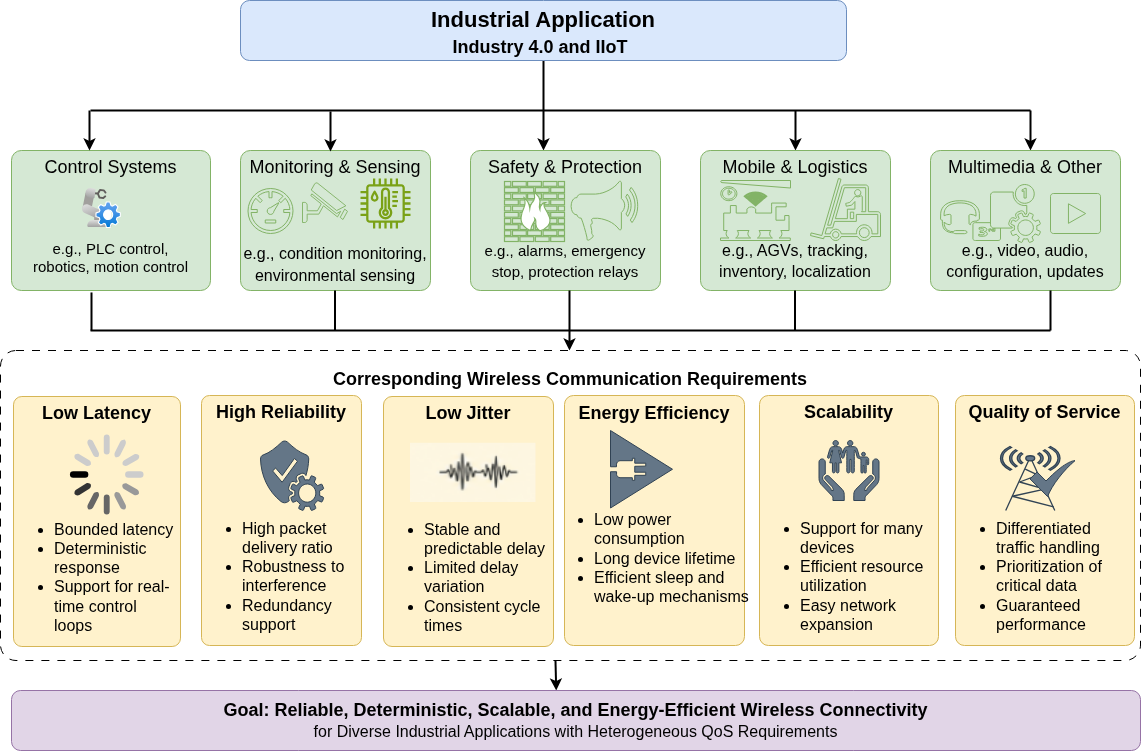
\includegraphics[width=\textwidth]{figures/IndustrialApp.png}
    \caption{Representative industrial applications and their corresponding
    wireless communication requirements.}
    \label{fig:industrial_requirements}
\end{figure*}

The evolution toward fifth-generation wireless communication broadened the scope of wireless systems beyond conventional human-centric broadband. The \gls{itur} IMT Vision defined three principal usage scenarios for \gls{imt2020}: enhanced mobile broadband, \gls{mmtc}, and \gls{urllc} \cite{itur_m2083}. The associated requirements and evaluation methodology cover performance dimensions such as latency, reliability, connection density, mobility, spectrum efficiency, and energy efficiency \cite{itur_m2410,itur_m2412}. Importantly, \gls{imt2020} is not restricted to a single radio interface; multiple \glspl{rit} can satisfy the common technical and evaluation framework \cite{itur_m2083,itur_m2410,itur_m2412,itur_m2150}.

This technology-neutral framework is particularly relevant to industrial and enterprise environments, where locally managed networks, flexible topologies, dense device connectivity, direct communication, and infrastructure-light deployment can be important. These requirements create a role for complementary radio technologies that address deployment models different from those of conventional cellular networks.

%%%%%%%%%%%%%%%%%%%%%%%%%%%%%%%%%%%%%%%%%%%%%%%%%%%%%%%%%%%%%%%%%%%%%%%%%%%%%%%% \subsection{DECT-2020 NR and the Emerging Research Landscape} \label{subsec:dectnr_landscape} %%%%%%%%%%%%%%%%%%%%%%%%%%%%%%%%%%%%%%%%%%%%%%%%%%%%%%%%%%%%%%%%%%%%%%%%%%%%%%%%

Within this context, \gls{etsi} developed \gls{dectnr} as a next-generation radio technology for local wireless communication, massive machine-type connectivity, and other demanding communication scenarios. Although it builds on the regulatory and technological heritage of \gls{dect}, \gls{dectnr} introduces a new radio interface and protocol architecture supporting flexible, decentralized, and infrastructure-light deployments \cite{kovalchukovDECT2020NewRadio2022, perez-guiraoDECTNRUnveiling2022}.

The technology was evaluated within the \gls{imt2020} process and subsequently included by the \gls{itur} as an \gls{imt2020} radio interface \cite{itur_m2150, maliatsosEvaluationIMT2020Candidate2022a, smidaETSIDECT2020Component2023}. Its architecture is specified primarily through the \gls{etsi} TS~103~636 series, covering the system architecture, radio requirements, \gls{phy}, \gls{mac}, and related protocol procedures \cite{etsi_ts103636_1, etsi_ts103636_2, etsi_ts103636_3, etsi_ts103636_4, etsi_ts103636_5}. Devices can assume different operational roles and establish direct, point-to-multipoint, and multi-hop communication structures without requiring the conventional base-station and core-network architecture associated with cellular systems.

These characteristics make \gls{dectnr} relevant to industrial and \gls{iot} environments in which local network ownership, deployment flexibility, device density, multi-hop connectivity, and application-specific communication requirements are important. Rather than being considered a replacement for cellular 5G, \gls{dectnr} can be viewed as a complementary \gls{imt2020} radio technology addressing deployment scenarios with distinct architectural and operational requirements \cite{kovalchukovDECT2020NewRadio2022, perez-guiraoDECTNRUnveiling2022, smidaETSIDECT2020Component2023}.

Research on \gls{dectnr} has expanded rapidly beyond standardization and initial technology evaluation. Early investigations concentrated on \gls{imt2020} performance assessment and the feasibility of the technology for machine-type and low-latency communication \cite{maliatsosEvaluationIMT2020Candidate2022a, smidaETSIDECT2020Component2023}. Subsequent work has addressed physical-layer performance, channel access, routing and multi-hop networking, scheduling and resource allocation, reliability, energy efficiency, positioning, coexistence, heterogeneous-network integration, and application-specific communication.

At the same time, evaluation has increasingly progressed from analytical and simulation-based studies toward commercial devices, hardware prototypes, \gls{sdr} implementations, testbeds, and measurements under practical deployment conditions \cite{fagerholmFPGAbasedDECT2020New2024, wassmannPerformanceDECT2020NR2024, bandaraExperimentalValidationAnalysis2025, haqueDECT2020NRLink2025, grafWhatExpectWhen2026}. Application-oriented research has similarly expanded toward professional audio, industrial monitoring, critical infrastructure, localization, energy-constrained networking, multi-hop communication, and other emerging use cases. This diversification suggests increasing research and experimental maturity, but it has also produced a fragmented research landscape spanning multiple protocol layers, methodologies, performance metrics, implementation platforms, and application domains.

%%%%%%%%%%%%%%%%%%%%%%%%%%%%%%%%%%%%%%%%%%%%%%%%%%%%%%%%%%%%%%%%%%%%%%%%%%%%%%%%
\subsection{Research Gap and Contributions}
\label{subsec:intro_gap}
%%%%%%%%%%%%%%%%%%%%%%%%%%%%%%%%%%%%%%%%%%%%%%%%%%%%%%%%%%%%%%%%%%%%%%%%%%%%%%%%

Despite this growing body of research, the available knowledge remains distributed across heterogeneous sources. Normative aspects are defined in \gls{etsi} specifications and \gls{itur} recommendations, whereas protocol enhancements, analytical models, simulations, implementation techniques, hardware evaluations, and application studies are distributed across journal articles, conference proceedings, theses, and other technical publications. Individual studies consequently provide detailed evidence for particular aspects of \gls{dectnr}, but do not by themselves reveal how the different research directions relate to one another, how experimental maturity has evolved, or where the principal research gaps remain.

Existing surveys and overview publications provide valuable descriptions of selected aspects of the technology \cite{kovalchukovDECT2020NewRadio2022, perez-guiraoDECTNRUnveiling2022, smidaETSIDECT2020Component2023}, but a systematic synthesis spanning the complete research landscape remains lacking. In particular, the literature has not yet been consolidated within a common framework that jointly characterizes publication trends, technical research areas, evaluation methodologies, implementation platforms, performance metrics, application domains, and cross-layer relationships.

This paper addresses this gap through a \gls{prisma}-based systematic literature review and technical synthesis of \gls{dectnr} research published from 2020 through July~2026 \cite{pagePRISMA2020}. Following systematic identification, screening, eligibility assessment, and quality assessment, 51 primary studies are included in the quantitative and qualitative synthesis. Normative \gls{etsi} and \gls{itur} documents are analyzed separately to provide the standardization context without treating standards as evaluation studies.

The principal contributions of this survey are as follows:

\begin{itemize}

    \item \textbf{Systematic and reproducible literature review:}     A structured review of the \gls{dectnr} literature is conducted using     predefined research questions, information sources, search strategy,     eligibility criteria, quality assessment, data extraction, and synthesis     procedures.

    \item \textbf{Quantitative characterization of the research landscape:}     The 51 primary studies are analyzed with respect to publication trends,     publication types, primary contributions, technical topics, research     methodologies, validation approaches, performance metrics, and     implementation platforms.

    \item \textbf{Unified technical taxonomy and synthesis:}     The research landscape is organized into ten complementary areas:     standardization and system architecture; physical-layer research;     \gls{mac} and channel access; routing and mesh networking; scheduling and     resource allocation; reliability, \gls{urllc}, and \gls{mmtc}; energy     efficiency; positioning and localization; security, coexistence, and     multi-RAT integration; and industrial applications and experimental     implementations.

    \item \textbf{Assessment of experimental maturity and performance     evaluation:}     The survey examines how \gls{dectnr} has been evaluated through analytical     modeling, simulation, hardware prototypes, commercial devices,     \gls{sdr} platforms, field trials, and industrial measurements, together     with the \glspl{kpi} used to characterize performance.

    \item \textbf{Cross-layer synthesis of technical evidence:}     Relationships among physical-layer configuration, channel access,     scheduling, routing, reliability, energy consumption, positioning, and     hardware behavior are synthesized to show how application-visible     performance emerges from interactions across protocol and implementation     layers.

    \item \textbf{Research gaps and future directions:}     Based on the systematic evidence, the survey identifies underexplored     areas and future priorities, including application-oriented cross-layer     design, large-scale mesh evaluation, deterministic communication,     energy-aware networking, experimental localization, secure multi-hop     operation, heterogeneous integration, and hardware-aware optimization.

\end{itemize}

By combining quantitative characterization with technical and cross-layer synthesis, this review provides a structured view of the maturity, limitations, and future development of the \gls{dectnr} research ecosystem.

%%%%%%%%%%%%%%%%%%%%%%%%%%%%%%%%%%%%%%%%%%%%%%%%%%%%%%%%%%%%%%%%%%%%%%%%%%%%%%%%
\subsection{Paper Organization}
\label{subsec:paper_organization}
%%%%%%%%%%%%%%%%%%%%%%%%%%%%%%%%%%%%%%%%%%%%%%%%%%%%%%%%%%%%%%%%%%%%%%%%%%%%%%%%

The remainder of this paper is organized as follows. Section~\ref{sec:methodology} describes the systematic review methodology, including the research questions, information sources, search strategy, eligibility criteria, quality assessment, data extraction, and synthesis procedure. Section~\ref{sec:results} presents the study-selection results and the quantitative characteristics of the 51 included primary studies. Section~\ref{sec:technical_synthesis} develops the technical taxonomy and synthesizes the major research directions across the ten identified areas. Section~\ref{sec:discussion} discusses the cross-layer implications, experimental and methodological limitations, research gaps, and future priorities. The final section concludes the paper.
%%%%%%%%%%%%%%%%%%%%%%%%%%%%%%%%%%%%%%%%%%%%%%%%%%%%%%%%%%%%%%%%%%%%%%%%%%%%%%%%
\section{Methodology}
\label{sec:methodology}
%%%%%%%%%%%%%%%%%%%%%%%%%%%%%%%%%%%%%%%%%%%%%%%%%%%%%%%%%%%%%%%%%%%%%%%%%%%%%%%%

This study adopts a \gls{slr} methodology following the \gls{prisma} 2020 guidelines \cite{pagePRISMA2020} to systematically identify, evaluate, classify, and synthesize the available literature on \gls{dectnr}. A predefined review protocol was established prior to the literature search to improve the transparency, consistency, and reproducibility of the review process.

As illustrated in Fig.~\ref{fig:review_workflow}, the review comprised four principal phases: identification, screening, eligibility assessment, and evidence synthesis. The identification phase covered the formulation of the \glspl{rq}, selection of information sources, development of the search strategy, literature retrieval, and duplicate removal. Screening was performed using titles and abstracts, followed by full-text eligibility assessment and \gls{qa}. The final phase comprised structured data extraction, classification, and synthesis of the included evidence.

\begin{figure*}[!t]
    \centering
    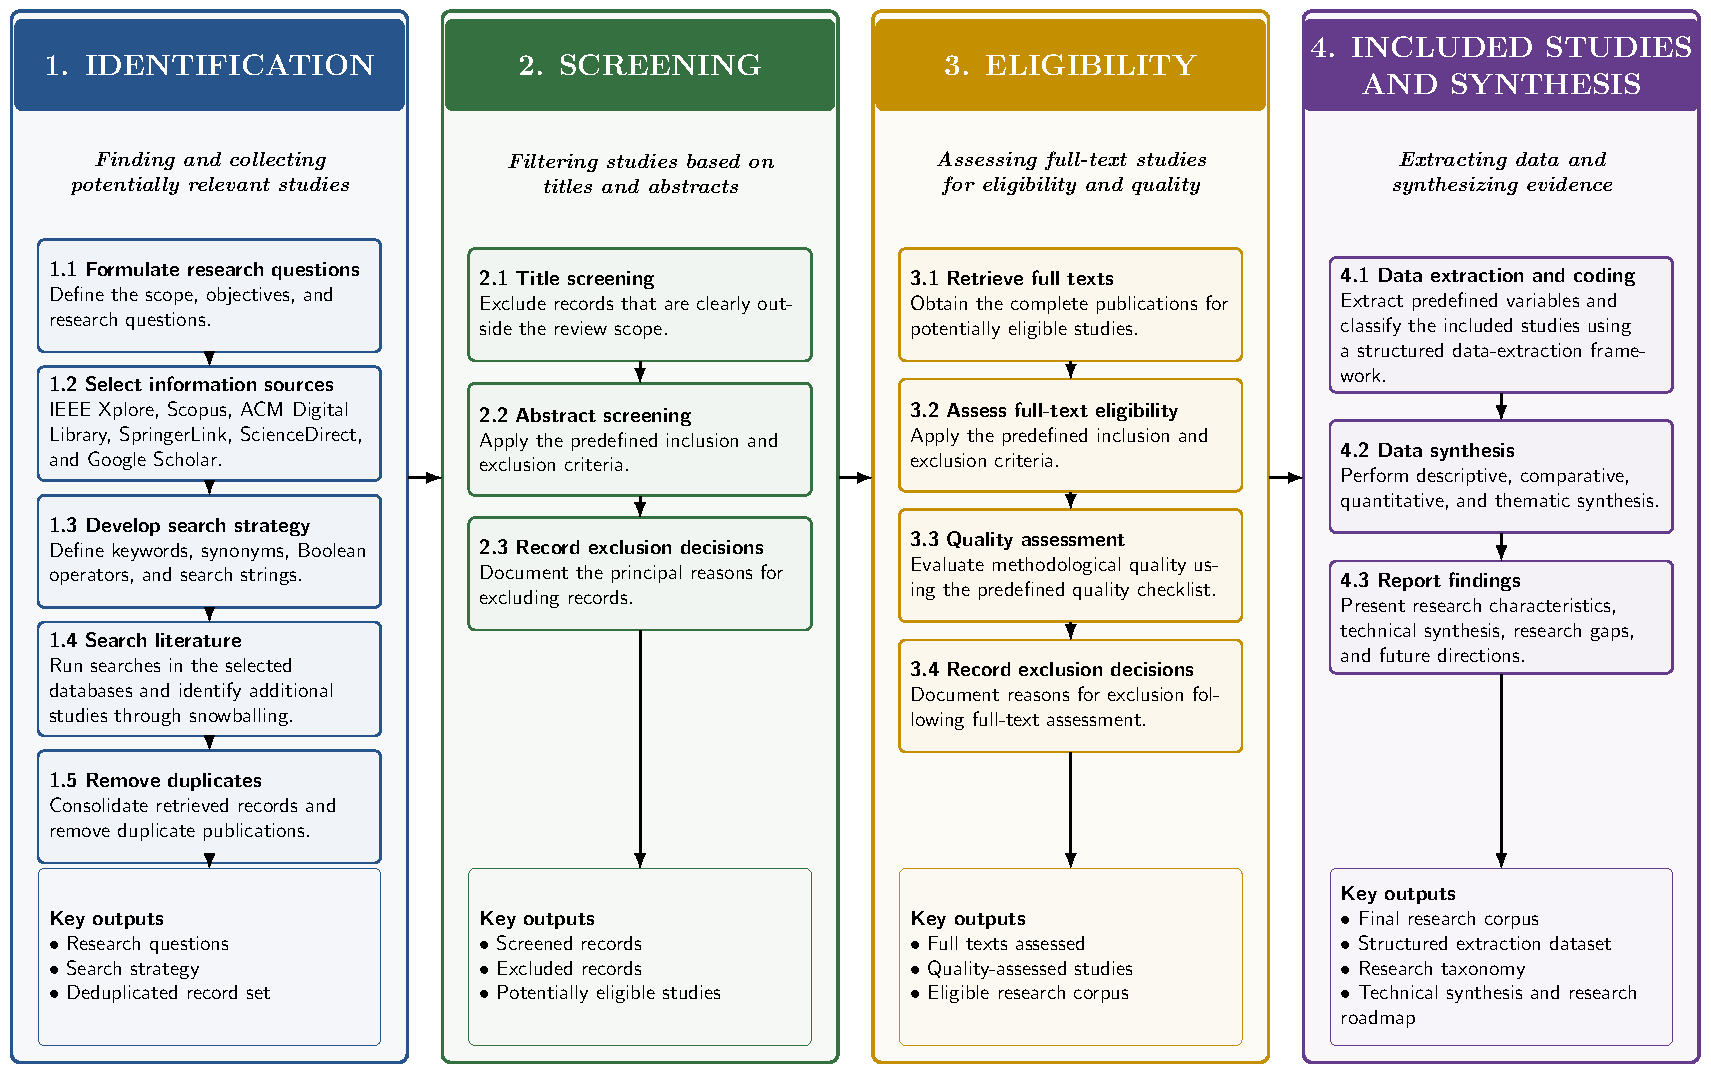
\includegraphics[width=\textwidth]{figures/PRSIMA.pdf}
    \caption{Systematic literature review workflow adopted in this study.
    The review comprises four principal phases: identification, screening,
    eligibility assessment, and evidence synthesis.}
    \label{fig:review_workflow}
\end{figure*}

%%%%%%%%%%%%%%%%%%%%%%%%%%%%%%%%%%%%%%%%%%%%%%%%%%%%%%%%%%%%%%%%%%%%%%%%%%%%%%%%
\subsection{Review Protocol and Research Questions}
\label{subsec:review_protocol}
%%%%%%%%%%%%%%%%%%%%%%%%%%%%%%%%%%%%%%%%%%%%%%%%%%%%%%%%%%%%%%%%%%%%%%%%%%%%%%%%

The review protocol defined the research objectives, information sources, search strategy, eligibility criteria, quality assessment procedure, data extraction framework, classification scheme, and synthesis methodology. The literature search covered publications from January 2020 to July 2026, corresponding to the emergence and subsequent development of \gls{dectnr}.

The review was guided by the following \glspl{rq}:

\begin{itemize}

    \item[\textbf{RQ1}] How has research on \gls{dectnr} evolved in terms of publication trends, publication types, and application domains?

    \item[\textbf{RQ2}] Which technical aspects of \gls{dectnr}, including the \gls{phy}, \gls{mac}, routing and mesh networking, resource allocation     and scheduling, positioning, security, and industrial applications, have     been investigated?

    \item[\textbf{RQ3}] Which evaluation methodologies, implementation platforms, software tools, and hardware platforms have been employed to  investigate and validate \gls{dectnr}?

    \item[\textbf{RQ4}] Which \glspl{kpi} have been used to evaluate \gls{dectnr}, and which performance characteristics have received the     greatest research attention?

    \item[\textbf{RQ5}] What are the principal scientific contributions and technical limitations reported in the existing literature?

    \item[\textbf{RQ6}] Which research gaps remain insufficiently addressed in the current body of \gls{dectnr} literature?

    \item[\textbf{RQ7}] What future research directions are most promising for advancing \gls{dectnr} toward large-scale \gls{iiot} deployments?

\end{itemize}

%%%%%%%%%%%%%%%%%%%%%%%%%%%%%%%%%%%%%%%%%%%%%%%%%%%%%%%%%%%%%%%%%%%%%%%%%%%%%%%% 
\subsection{Information Sources and Search Strategy}
\label{subsec:search_strategy}
%%%%%%%%%%%%%%%%%%%%%%%%%%%%%%%%%%%%%%%%%%%%%%%%%%%%%%%%%%%%%%%%%%%%%%%%%%%%%%%%

The literature search was conducted using five primary scientific databases: IEEE Xplore, Scopus, ACM Digital Library, SpringerLink, and ScienceDirect. Google Scholar was used as a complementary source for backward and forward snowballing and for identifying potentially relevant publications not retrieved through the primary database search.

To capture both technology-specific publications and studies addressing its main technical and application-oriented aspects, the search strategy combined alternative names for \gls{dectnr} with terms related to architecture, protocol design, the \gls{phy}, the \gls{mac}, implementation, experimental validation, performance evaluation, and industrial communication. The Boolean search query used in the review was:

\begin{quote} \small \texttt{ ("DECT-2020 NR" OR "DECT NR+" OR "DECT-2020 New Radio" OR "DECT NR" OR "DECT New Radio") AND (architecture OR protocol OR PHY OR "physical layer" OR MAC OR "medium access control" OR implementation OR experimental OR testbed OR prototype OR performance OR evaluation OR measurement OR industrial OR IoT OR URLLC OR reliability) }
\end{quote}

Database-specific syntax was adapted where necessary while preserving the semantic meaning of the search expression. Where supported by the respective database, the search was applied to publication titles, abstracts, and author-defined keywords.

All retrieved records were consolidated and managed using Zotero Reference Manager. Duplicate records were identified and removed before the screening stage. Backward snowballing was performed by examining the references of eligible studies, while forward snowballing was supported using Google Scholar. Additional studies identified through snowballing were subjected to the same eligibility criteria as records retrieved through the primary search.

Normative \gls{etsi} specifications, \gls{etsi} Technical Reports, and relevant \gls{itur} recommendations were additionally consulted to establish the standardization and technical baseline for the synthesis. These normative documents were analyzed separately from the primary research corpus and were therefore not included in the quantitative bibliometric analysis or subjected to the research-study quality assessment procedure.

%%%%%%%%%%%%%%%%%%%%%%%%%%%%%%%%%%%%%%%%%%%%%%%%%%%%%%%%%%%%%%%%%%%%%%%%%%%%%%%%
\subsection{Eligibility and Study Selection}
\label{subsec:eligibility}
%%%%%%%%%%%%%%%%%%%%%%%%%%%%%%%%%%%%%%%%%%%%%%%%%%%%%%%%%%%%%%%%%%%%%%%%%%%%%%%%

The inclusion and exclusion criteria were defined before screening. A study was eligible for the primary research corpus if it:

\begin{itemize}

    \item primarily investigated \gls{dectnr} or DECT NR+;

    \item presented a technical, analytical, experimental, architectural, or     application-oriented contribution;

    \item was written in English and had accessible full text;

    \item was published between January 2020 and July 2026; and

    \item contained sufficient methodological or technical information for     data extraction.

\end{itemize}

Studies were excluded if they mentioned \gls{dectnr} only as background, primarily investigated another communication technology, duplicated another record, lacked sufficient technical content, or consisted of non-technical material such as presentation slides, posters, or editorials.

Studies relevant to the broader technological context but not primarily focused on \gls{dectnr} were classified as contextual studies and excluded from the quantitative synthesis.

Study selection was performed sequentially through title screening, abstract screening, and full-text eligibility assessment. Exclusion decisions were recorded throughout the screening process. The numerical outcome of the study selection procedure is reported separately using the \gls{prisma} flow diagram in Section~\ref{sec:results}.

%%%%%%%%%%%%%%%%%%%%%%%%%%%%%%%%%%%%%%%%%%%%%%%%%%%%%%%%%%%%%%%%%%%%%%%%%%%%%%%%
\subsection{Quality Assessment}
\label{subsec:quality_assessment}
%%%%%%%%%%%%%%%%%%%%%%%%%%%%%%%%%%%%%%%%%%%%%%%%%%%%%%%%%%%%%%%%%%%%%%%%%%%%%%%%

Eligible research studies were evaluated using a five-criterion \gls{qa} framework covering:

\begin{enumerate}

    \item clarity of the research objective;

    \item appropriateness of the methodology;

    \item strength of the validation;

    \item clarity of the discussion and limitations; and

    \item reproducibility of the study.

\end{enumerate}

Each criterion was assigned a score of 0 (not addressed), 1 (partially addressed), or 2 (fully addressed), resulting in a maximum quality score of 10. Studies scoring 8--10 were classified as high quality, those scoring 5--7 as moderate quality, and those scoring below 5 as low quality. No study was excluded solely on the basis of its quality score; rather, the quality assessment was used to characterize the methodological strength of the evidence and to support interpretation of the synthesized findings.

%%%%%%%%%%%%%%%%%%%%%%%%%%%%%%%%%%%%%%%%%%%%%%%%%%%%%%%%%%%%%%%%%%%%%%%%%%%%%%%%
\subsection{Data Extraction and Coding}
\label{subsec:data_extraction}
%%%%%%%%%%%%%%%%%%%%%%%%%%%%%%%%%%%%%%%%%%%%%%%%%%%%%%%%%%%%%%%%%%%%%%%%%%%%%%%%

A structured data-extraction template was used to ensure consistent collection of information from the included studies. The extracted variables covered bibliographic characteristics, research contributions, technical topics, evaluation methodologies, implementation platforms, deployment characteristics, evaluated \glspl{kpi}, application domains, key findings, limitations, identified research gaps, and proposed future work.

Each publication was assigned one primary research contribution to avoid double counting in the analysis of dominant research directions. Secondary technical characteristics were coded using a multi-label classification scheme covering the \gls{phy}, \gls{mac}, routing and mesh networking, scheduling and resource allocation, positioning and localization, security, energy efficiency, coexistence, artificial intelligence, industrial applications, \gls{urllc}, \gls{mmtc}, and related topics.

Evaluation methodologies and reported performance metrics were also treated as multi-label variables because individual studies frequently employed multiple evaluation approaches or investigated several \glspl{kpi}. Binary one-hot coding was used for these attributes in the structured spreadsheet database.

To improve consistency, the extracted data and corresponding classification matrices were cross-checked against the source publications. Ambiguous or inconsistent classifications were resolved by re-examining the relevant sections of the full text. Following verification, the resulting database was frozen and used as the single source for the quantitative analyses, tables, and figures reported in this review.

%%%%%%%%%%%%%%%%%%%%%%%%%%%%%%%%%%%%%%%%%%%%%%%%%%%%%%%%%%%%%%%%%%%%%%%%%%%%%%%%
\subsection{Data Synthesis and Threats to Validity}
\label{subsec:data_synthesis}
%%%%%%%%%%%%%%%%%%%%%%%%%%%%%%%%%%%%%%%%%%%%%%%%%%%%%%%%%%%%%%%%%%%%%%%%%%%%%%%%

The extracted evidence was analyzed using descriptive, comparative, and thematic synthesis. Descriptive analysis was used to characterize publication trends, publication types, research topics, evaluation methodologies, implementation platforms, application domains, and reported performance metrics. Comparative analysis was used to examine methodological and technical differences across the identified research categories. Thematic synthesis was subsequently applied to integrate scientific contributions, limitations, research gaps, and proposed future directions across the literature.

Because several variables, including technical topics, evaluation methods, and performance metrics, were coded using a multi-label scheme, the sum of the corresponding category frequencies or percentages may exceed the total number of publications or 100\%.

Several threats to validity remain. Relevant studies may have been missed because of differences in database coverage, indexing, or terminology. This risk was mitigated through searches across multiple scientific databases and backward and forward snowballing. Classification and quality assessment also involve researcher judgment. To reduce subjectivity, predefined coding and assessment criteria were applied consistently, and ambiguous classifications were re-examined against the corresponding full-text publications. Finally, \gls{dectnr} remains a rapidly evolving technology, and recently accepted or unpublished studies may not yet be indexed. Consequently, the review represents the state of the literature available up to July 2026.
%%%%%%%%%%%%%%%%%%%%%%%%%%%%%%%%%%%%%%%%%%%%%%%%%%%%%%%%%%%%%%%%%%%%%%%%%%%%%%%%
\section{Results of the Systematic Literature Review}
\label{sec:results}
%%%%%%%%%%%%%%%%%%%%%%%%%%%%%%%%%%%%%%%%%%%%%%%%%%%%%%%%%%%%%%%%%%%%%%%%%%%%%%%%

This section presents the quantitative results of the systematic literature review. The analysis characterizes the study-selection process, publication trends, technical research distribution, evaluation methodologies, validation approaches, reported performance metrics, and implementation platforms. The technical contributions and findings of the individual studies are not examined in detail here; instead, they are synthesized thematically in the subsequent technical synthesis section.

%%%%%%%%%%%%%%%%%%%%%%%%%%%%%%%%%%%%%%%%%%%%%%%%%%%%%%%%%%%%%%%%%%%%%%%%%%%%%%%%
\subsection{Study Selection and Search Results}
\label{subsec:study_selection_results}
%%%%%%%%%%%%%%%%%%%%%%%%%%%%%%%%%%%%%%%%%%%%%%%%%%%%%%%%%%%%%%%%%%%%%%%%%%%%%%%%

The systematic literature search was conducted in July 2026 according to the review protocol described in Section~\ref{sec:methodology}. Searches across the five primary literature databases identified 107 records in total: 42 from IEEE Xplore, 44 from Scopus, one from the ACM Digital Library, 15 from SpringerLink, and five from ScienceDirect. In addition to the primary database search, Google Scholar was used to support backward and forward citation searching. This complementary snowballing process involved the examination of 226 records.

Combining the primary database search and the records examined through snowballing resulted in 333 records at the identification stage. Duplicate and other records that did not proceed to formal screening were removed before screening, leaving 86 records for title and abstract assessment. At this stage, 22 records were excluded, and 64 reports were subsequently sought for full-text retrieval. Five reports could not be retrieved, resulting in 59 reports being assessed for full-text eligibility according to the predefined criteria described in Section~\ref{subsec:eligibility}.

Of the 59 reports assessed at the full-text stage, 51 satisfied the criteria for inclusion in the primary research corpus and were retained for the quantitative synthesis. The remaining eight records did not form part of the primary corpus: five were retained as contextual or background studies, two were excluded because their primary technical focus was not \gls{dectnr}, and one duplicate was identified during final verification. Accordingly, the quantitative analyses presented in the remainder of this section are based on the 51 included studies.

Normative \gls{etsi} specifications, \gls{etsi} Technical Reports, and relevant \gls{itur} recommendations were consulted separately to establish the technical and standardization baseline. As specified in the review methodology, these documents were not treated as primary research studies and were therefore not included in the 51-study quantitative corpus.

The complete study-selection process is summarized in the \gls{prisma} flow diagram shown in Fig.~\ref{fig:prisma_results}.

\begin{figure}[!t]
    \centering
    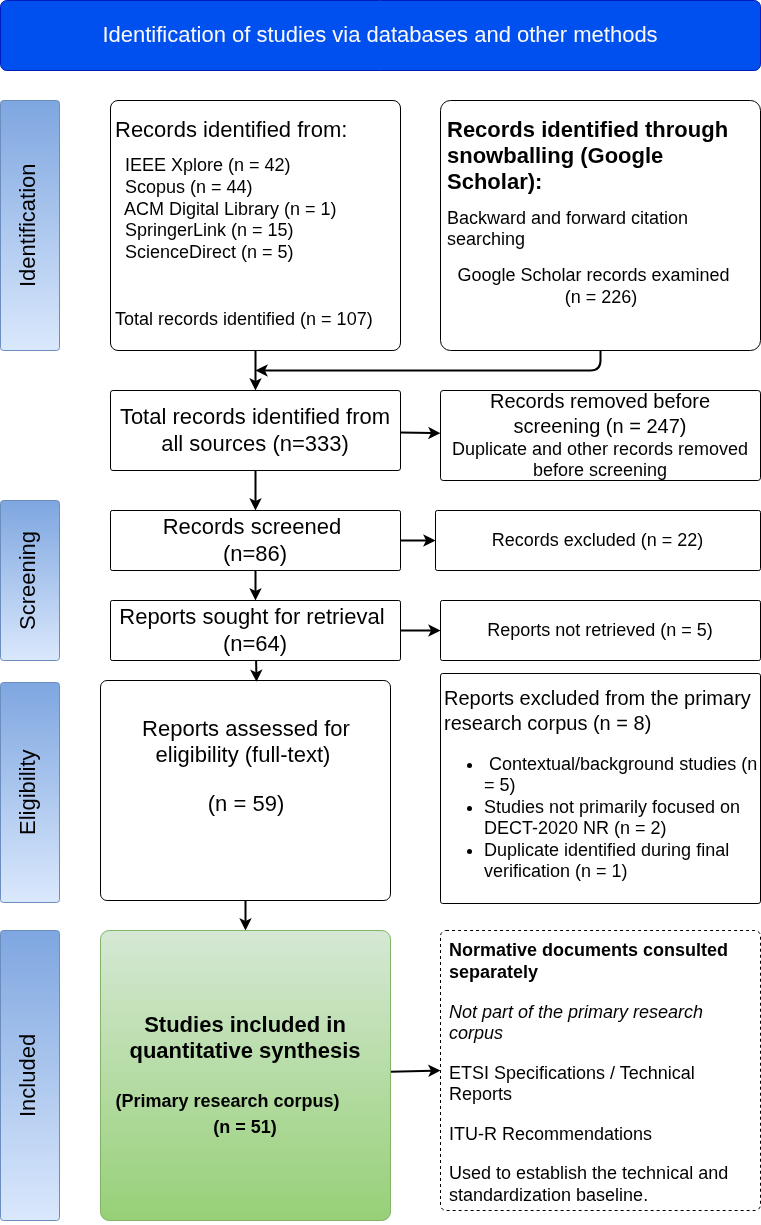
\includegraphics[width=\columnwidth]{figures/PRISMA_Result.png}
    \caption{PRISMA flow diagram of the study identification, screening,
    eligibility assessment, and final inclusion process.}
    \label{fig:prisma_results}
\end{figure}

%%%%%%%%%%%%%%%%%%%%%%%%%%%%%%%%%%%%%%%%%%%%%%%%%%%%%%%%%%%%%%%%%%%%%%%%%%%%%%%%
\subsection{Research Characteristics}
\label{subsec:research_characteristics}
%%%%%%%%%%%%%%%%%%%%%%%%%%%%%%%%%%%%%%%%%%%%%%%%%%%%%%%%%%%%%%%%%%%%%%%%%%%%%%%%

The final research corpus comprises 51 studies published between 2020 and July 2026. Fig.~\ref{fig:publication_year} shows the annual distribution of the included studies. Research activity was initially limited, with one included study in 2020, followed by four studies in 2021, five in 2022, and three in 2023. Publication activity increased substantially thereafter, reaching 13 studies in 2024 and 16 studies in 2025. A further nine studies were identified in 2026 up to the review cut-off in July.

\begin{figure}[!t]
    \centering
    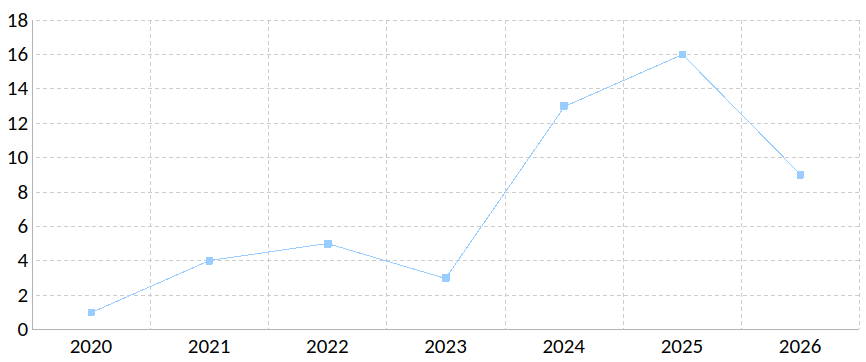
\includegraphics[width=\columnwidth]{figures/fig1.png}
    \caption{Annual distribution of the 51 included \gls{dectnr} studies
    published between 2020 and July 2026.}
    \label{fig:publication_year}
\end{figure}

The temporal distribution shows a marked increase in research activity from 2024 onward. Of the 51 included studies, 38 were published between 2024 and July 2026, representing approximately 75\% of the primary research corpus. The lower number observed for 2026 should be interpreted in relation to the July 2026 search cut-off and therefore does not represent a complete publication year.

Fig.~\ref{fig:publication_type} presents the distribution of the included studies by publication type. Conference papers constitute the dominant publication channel, accounting for 36 of the 51 studies (70.6\%). The remaining corpus comprises seven survey or overview papers (13.7\%), five journal articles (9.8\%), and three theses (5.9\%).

\begin{figure}[!t]
    \centering
    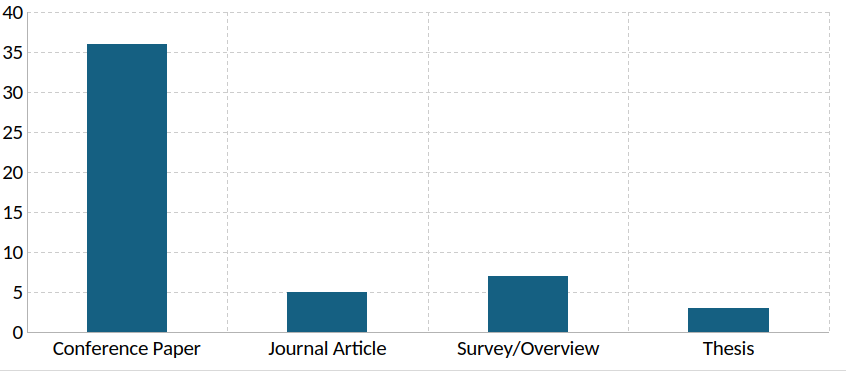
\includegraphics[width=\columnwidth]{figures/fig2.png}
    \caption{Distribution of the 51 included studies by publication type.}
    \label{fig:publication_type}
\end{figure}

The publication distribution is therefore characterized by a strong concentration of conference papers and a substantial increase in publication activity from 2024 onward. Journal publications remain comparatively limited, whereas survey and overview papers constitute a smaller but noticeable component of the literature.

%%%%%%%%%%%%%%%%%%%%%%%%%%%%%%%%%%%%%%%%%%%%%%%%%%%%%%%%%%%%%%%%%%%%%%%%%%%%%%%%
\subsection{Technical Research Landscape}
\label{subsec:technical_landscape}
%%%%%%%%%%%%%%%%%%%%%%%%%%%%%%%%%%%%%%%%%%%%%%%%%%%%%%%%%%%%%%%%%%%%%%%%%%%%%%%%

To characterize the technical orientation of the literature, each included study was assigned one primary contribution category representing its dominant research focus. Fig.~\ref{fig:primary_contribution} presents the resulting distribution across the 51-study corpus.

\begin{figure}[!t]
    \centering
    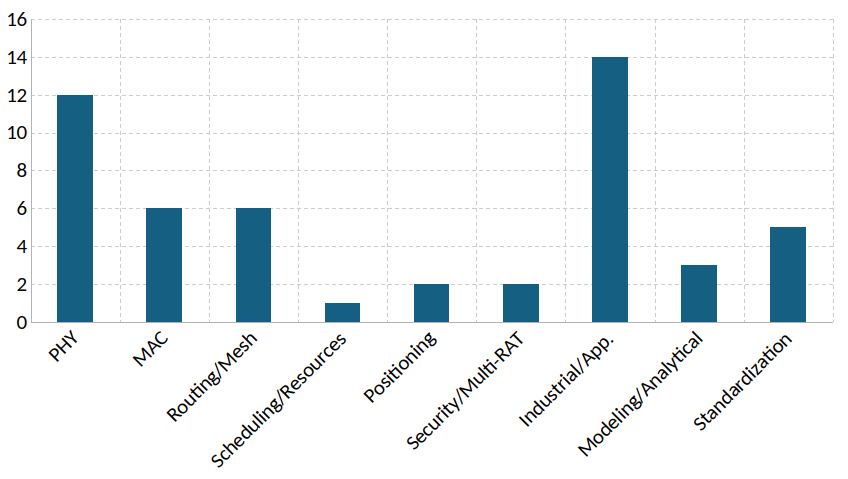
\includegraphics[width=\columnwidth]{figures/fig3.png}
    \caption{Distribution of the included studies according to their primary
    technical contribution.}
    \label{fig:primary_contribution}
\end{figure}

Industrial and application-oriented research constitutes the largest primary contribution category, accounting for 14 studies, followed by \gls{phy} research with 12 studies. \gls{mac} and routing or mesh-networking research each account for six studies, while five studies primarily address standardization. Modeling and analytical research accounts for three studies, whereas positioning and security or multi-RAT research each comprise two studies. Only one study was classified primarily under scheduling and resource allocation.

The primary-contribution classification assigns each study to a single dominant category and therefore provides a mutually exclusive view of the research corpus. However, many studies address several technical aspects simultaneously. To capture this overlap, the literature was additionally coded using multi-label technical-topic categories. The resulting distribution is shown in Fig.~\ref{fig:technical_topics}.

\begin{figure}[!t]
    \centering
    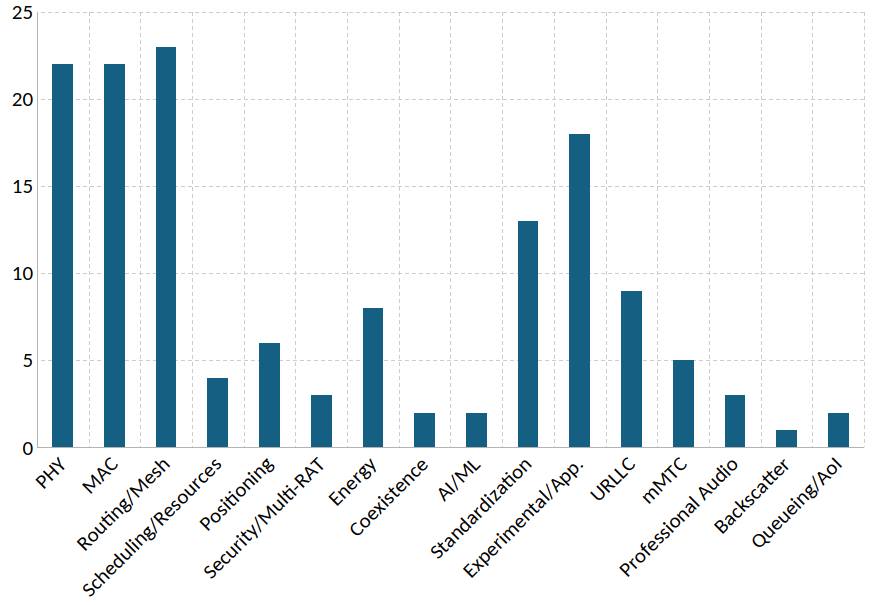
\includegraphics[width=\columnwidth]{figures/fig4.png}
    \caption{Technical topics addressed across the included studies.
    Multiple topics may be assigned to an individual study.}
    \label{fig:technical_topics}
\end{figure}

Routing and mesh networking is the most frequently represented technical topic, appearing in 23 studies, followed by \gls{phy} and \gls{mac} aspects with 22 studies each. Experimental, testbed, or application-oriented aspects are reported in 18 studies, while standardization or overview topics occur in 13 studies. Among the service-oriented topics, \gls{urllc} is addressed in nine studies and \gls{mmtc} in five. Energy-related aspects occur in eight studies and positioning in six, whereas scheduling and resource allocation appear in four studies.

Other topics remain less frequently represented: security or multi-RAT operation appears in three studies, professional audio in three, and coexistence or regulatory aspects, AI/ML, and queueing or Age of Information each occur in two studies. Backscatter or ambient-IoT communication appears in one study. Because this classification is multi-label, the category counts exceed the total number of included studies.

%%%%%%%%%%%%%%%%%%%%%%%%%%%%%%%%%%%%%%%%%%%%%%%%%%%%%%%%%%%%%%%%%%%%%%%%%%%%%%%%
\subsection{Evaluation Characteristics}
\label{subsec:evaluation_characteristics}
%%%%%%%%%%%%%%%%%%%%%%%%%%%%%%%%%%%%%%%%%%%%%%%%%%%%%%%%%%%%%%%%%%%%%%%%%%%%%%%%

The methodological characteristics of the literature were examined by classifying the evaluation approaches used by the included studies. Fig.~\ref{fig:evaluation_methodologies} summarizes the resulting distribution. Since individual studies may combine multiple evaluation approaches, these categories are not mutually exclusive.

\begin{figure}[!t]
    \centering
    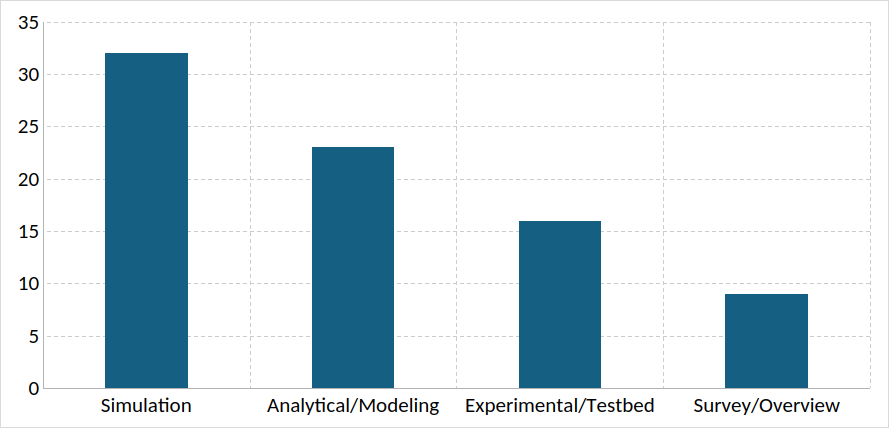
\includegraphics[width=\columnwidth]{figures/fig5.png}
    \caption{Evaluation methodologies employed across the included studies.
    Multiple methodologies may be reported by an individual study.}
    \label{fig:evaluation_methodologies}
\end{figure}

Simulation is the most frequently employed evaluation methodology, appearing in 32 studies, while analytical or modeling approaches are reported in 23 studies. Experimental or testbed-based evaluation is present in 16 studies, and nine studies employ survey or overview methodologies. The distribution therefore shows that simulation and analytical evaluation constitute a substantial component of the current evidence base, alongside an established body of experimental research.

Fig.~\ref{fig:validation_approaches} further distinguishes the specific validation approaches reported in the literature.

\begin{figure}[!t]
    \centering
    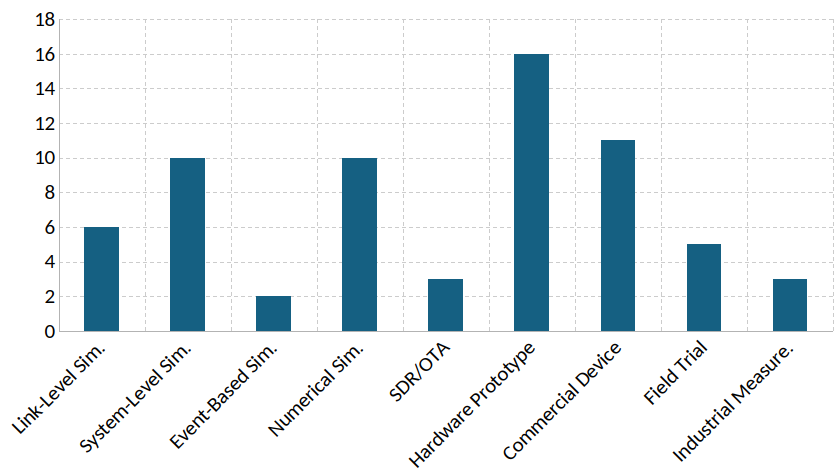
\includegraphics[width=\columnwidth]{figures/fig6.png}
    \caption{Validation approaches reported across the included studies.
    Multiple validation approaches may be associated with an individual study.}
    \label{fig:validation_approaches}
\end{figure}

Hardware prototypes represent the most frequently reported validation approach, appearing in 16 studies, followed by commercial-device evaluation in 11 studies. System-level and numerical simulation are each reported in 10 studies, while link-level simulation appears in six and event-based simulation in two. Among experimental approaches, five studies report field trials, three employ \gls{sdr} or over-the-air validation, and three report industrial measurements. These categories may overlap where studies combine simulation, prototype implementation, and experimental validation.

The performance indicators used to evaluate \gls{dectnr} are summarized in Fig.~\ref{fig:performance_metrics}. As with the preceding classifications, multiple metrics may be reported by a single study.

\begin{figure}[!t]
    \centering
    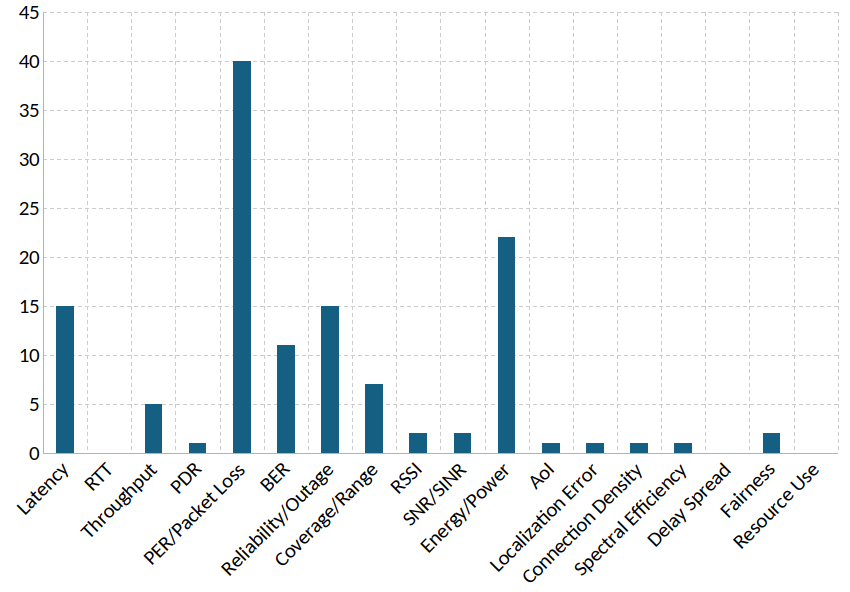
\includegraphics[width=\columnwidth]{figures/fig7.png}
    \caption{Performance metrics reported across the included studies.
    Multiple metrics may be reported by an individual study.}
    \label{fig:performance_metrics}
\end{figure}

Packet error rate or packet-loss-related metrics are the most frequently reported performance measures, occurring in 40 studies. Energy or power metrics are reported in 22 studies, while latency and reliability or outage metrics each appear in 15 studies. Bit error rate is reported in 11 studies, and coverage or communication range in seven. Throughput is evaluated in five studies, while RSSI, SNR/SINR, and fairness each occur in two studies. Packet delivery ratio, Age of Information, localization error, connection density, and spectral efficiency are each reported in one study. No studies in the coded corpus explicitly reported RTT, delay spread, or resource-use metrics as separate evaluation indicators.

Finally, Fig.~\ref{fig:implementation_platforms} summarizes the explicitly reported implementation and software platforms identified in the included studies.

\begin{figure}[!t]
    \centering
    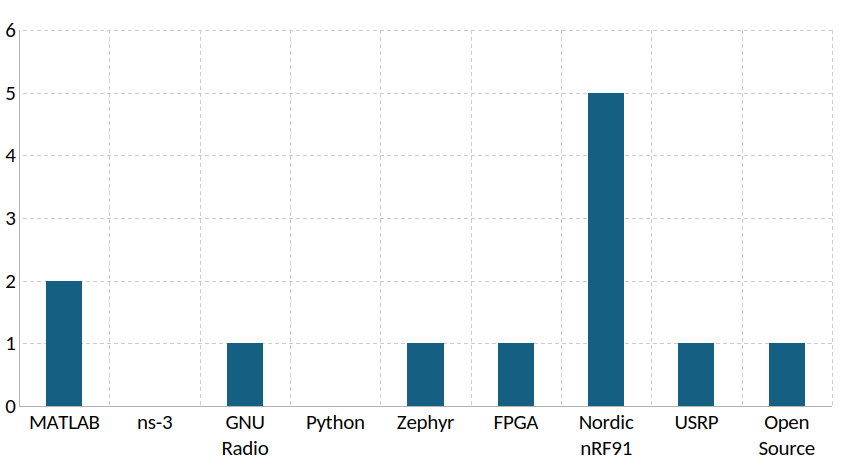
\includegraphics[width=\columnwidth]{figures/fig8.png}
    \caption{Software and hardware platforms explicitly reported across the
    included studies. Multiple platforms may be associated with an individual
    study.}
    \label{fig:implementation_platforms}
\end{figure}

Nordic nRF91-series hardware is the most frequently identified implementation platform, appearing in five studies. MATLAB is explicitly reported in two studies, while GNU Radio, Zephyr, FPGA-based platforms, USRP, and explicitly identified open-source implementations each occur in one study. No studies in the coded corpus explicitly identified ns-3 or Python as implementation platforms under the adopted coding scheme.

Overall, the quantitative results reveal a research landscape characterized by rapid recent publication growth, a strong concentration of conference papers, and substantial activity in \gls{phy}, \gls{mac}, routing and mesh networking, and industrial or application-oriented research. Simulation and analytical evaluation remain prominent, while hardware prototypes, commercial devices, field trials, and industrial measurements constitute an established experimental component of the literature. The technical implications of these distributions, including the maturity of individual research areas and the remaining gaps in the literature, are examined in the following technical synthesis section.
%%%%%%%%%%%%%%%%%%%%%%%%%%%%%%%%%%%%%%%%%%%%%%%%%%%%%%%%%%%%%%%%%%%%%%%%%%%%%%%%
\section{Technical Synthesis of DECT-2020 NR Research}
\label{sec:technical_synthesis}
%%%%%%%%%%%%%%%%%%%%%%%%%%%%%%%%%%%%%%%%%%%%%%%%%%%%%%%%%%%%%%%%%%%%%%%%%%%%%%%%

The quantitative results presented in Section~\ref{sec:results} describe the distribution of the reviewed literature across publication characteristics, technical topics, methodologies, and evaluation approaches. This section complements that quantitative analysis with a technical synthesis of the 51 included primary studies. Based on their principal technical contributions, the literature is organized into the research taxonomy shown in Fig.~\ref{fig:research_taxonomy}. The taxonomy provides the structure for the subsequent analysis while recognizing that individual studies may contribute to multiple research areas.

\begin{figure*}[!t]
    \centering
    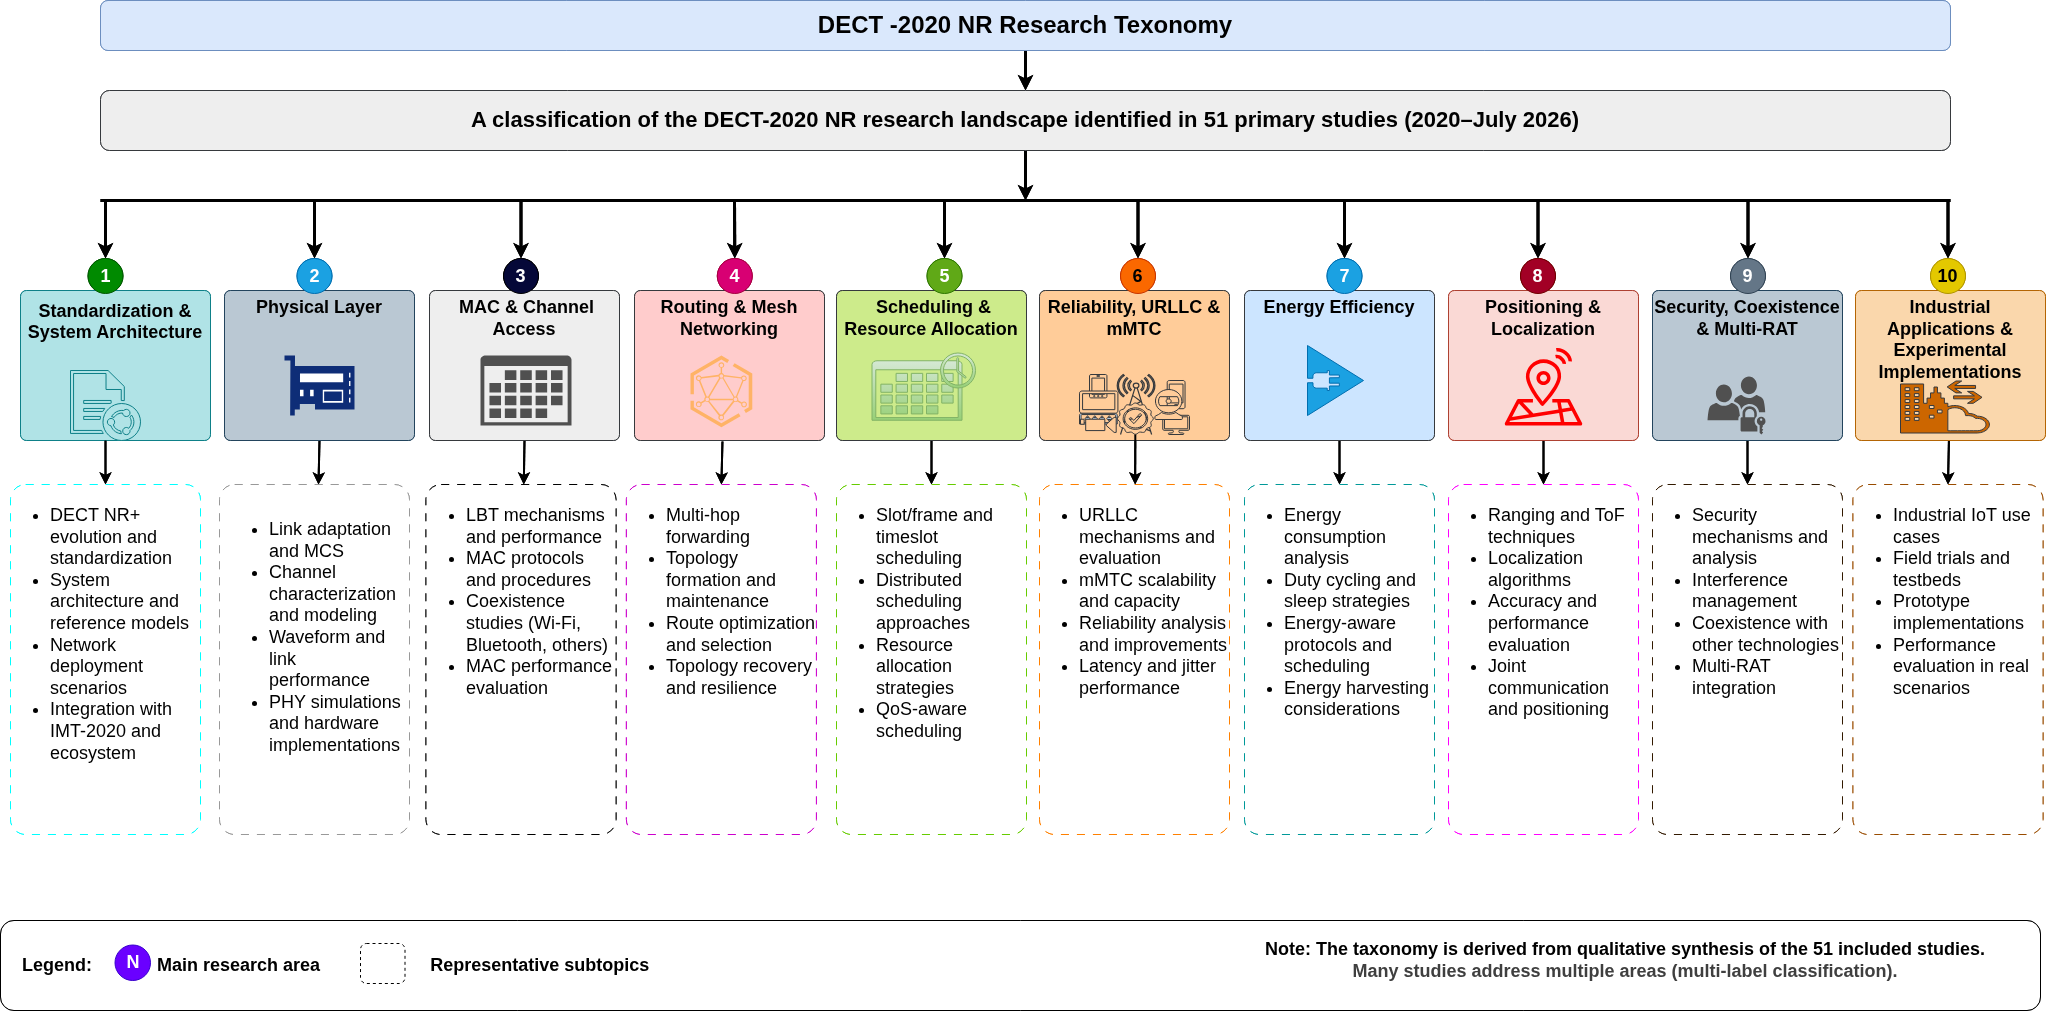
\includegraphics[width=\textwidth]{figures/ResearchTexanomy.png}
    \caption{Taxonomy of the DECT-2020 NR research landscape derived from the
    qualitative synthesis of the 51 included primary studies. The taxonomy
    organizes the literature into ten principal research areas while allowing
    individual studies to address multiple areas.}
    \label{fig:research_taxonomy}
\end{figure*}

%%%%%%%%%%%%%%%%%%%%%%%%%%%%%%%%%%%%%%%%%%%%%%%%%%%%%%%%%%%%%%%%%%%%%%%%%%%%%%%%
\subsection{Standardization and System Architecture}
\label{subsec:standardization_architecture}
%%%%%%%%%%%%%%%%%%%%%%%%%%%%%%%%%%%%%%%%%%%%%%%%%%%%%%%%%%%%%%%%%%%%%%%%%%%%%%%%

The standardization and architectural foundations of \gls{dectnr} provide the basis for subsequent research on the \gls{phy}, \gls{mac}, routing, resource management, and industrial applications. As shown in Section~\ref{subsec:technical_landscape}, five studies in the final corpus were classified primarily as standardization or overview contributions, while architectural aspects recur across several other technical categories \cite{kovalchukovDECT2020NewRadio2022, perez-guiraoDECTNRUnveiling2022, maliatsosEvaluationIMT2020Candidate2022a, smidaETSIDECT2020Component2023}.

The development of \gls{dectnr} was closely associated with the \gls{imt2020} standardization process. The \gls{itur} established the IMT-2020 vision, minimum performance requirements, and evaluation methodology through ITU-R M.2083, M.2410, and M.2412 \cite{itur_m2083,itur_m2410,itur_m2412}. DECT-2020 NR was subsequently evaluated as a candidate \gls{rit}, particularly for \gls{urllc} and \gls{mmtc}, and its inclusion in Recommendation ITU-R M.2150 established it as an IMT-2020 radio interface \cite{itur_m2150, maliatsosEvaluationIMT2020Candidate2022a, smidaETSIDECT2020Component2023}. Early studies therefore focused on specification-level evaluation and compliance with the IMT-2020 framework, providing the baseline for later protocol- and application-oriented research \cite{maliatsosEvaluationIMT2020Candidate2022a, smidaETSIDECT2020Component2023}.

The \gls{dectnr} specification is organized as a modular protocol family. ETSI TS~103~636-1 defines the general system description and terminology, Part~2 the radio requirements, Part~3 the \gls{phy}, Part~4 the \gls{mac}, and Part~5 the data-link-control and convergence functionality \cite{etsi_ts103636_1, etsi_ts103636_2, etsi_ts103636_3, etsi_ts103636_4, etsi_ts103636_5}. The specification framework has subsequently evolved through Release~2 revisions, extending the technical baseline while retaining the fundamental DECT NR+ system architecture \cite{etsi_ts_103636_1_r2, etsi_ts_103636_3_r2, etsi_ts_103636_4_r2}. Complementary technical reports document IMT-2020 evaluation and additional technical and regulatory aspects \cite{etsi_tr103810,etsi_tr103943,etsi_tr_103810}. Together, these specifications provide the protocol framework underlying the technical research synthesized in the following subsections.

Beyond introducing a new radio interface, \gls{dectnr} adopts a decentralized and flexible architecture designed for dense machine-type and vertical communication \cite{kovalchukovDECT2020NewRadio2022, perez-guiraoDECTNRUnveiling2022}. Montalvo et al. place this development within the broader evolution of the DECT family, from classical cordless communication and DECT-ULE toward the multicarrier, OFDM-based DECT-2020 NR interface developed for substantially different connectivity and performance requirements \cite{montalvoDECTEvolutionMeeting2024}.

A fundamental architectural element is the distinction between the logical \gls{ft} and \gls{pt} roles. An \gls{ft} provides control and radio-resource information, whereas \glspl{pt} discover and associate with an \gls{ft} and use the available communication resources. These are logical protocol roles rather than permanently assigned hardware classes, allowing devices to support different roles according to their network function \cite{etsi_ts103636_1, etsi_ts103636_4, kovalchukovDECT2020NewRadio2022, perez-guiraoDECTNRUnveiling2022}. This flexibility enables point-to-point and local-cluster communication as well as hierarchical and mesh-oriented multi-hop structures in which combined FT/PT devices extend connectivity without requiring every device to maintain a direct link to centralized infrastructure \cite{etsi_ts103636_1, etsi_ts103636_4, kovalchukovDECT2020NewRadio2022, perez-guiraoDECTNRUnveiling2022}.

\begin{figure*}[!t]
    \centering
    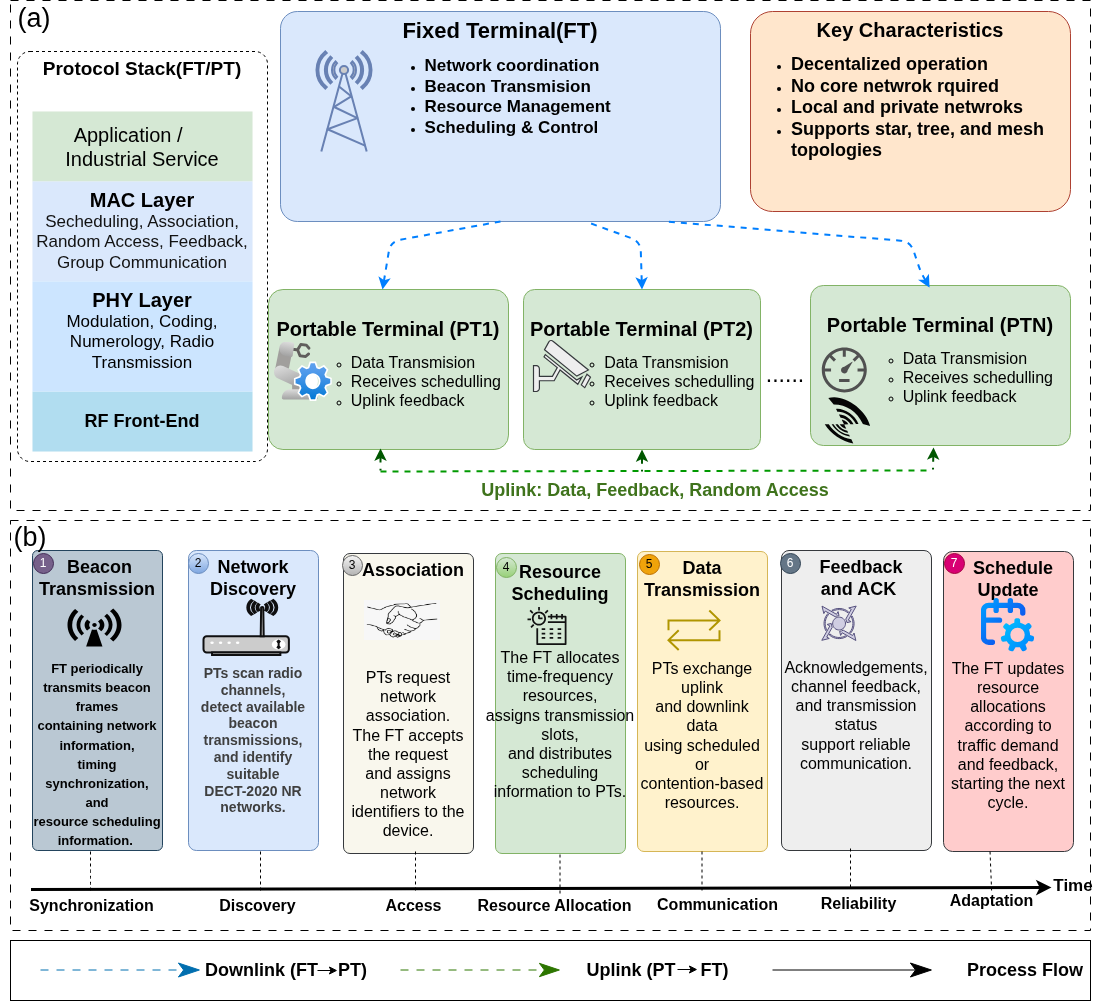
\includegraphics[width=0.95\textwidth]{figures/archetictur.png}
    \caption{Conceptual \gls{dectnr} architecture and representative
    communication workflow, illustrating logical FT/PT roles, network
    formation, resource coordination, association, data transmission, and
    feedback procedures.}
    \label{fig:dectnr_architecture}
\end{figure*}

Network formation is supported through standardized discovery, beaconing, association, random-access, and resource-allocation procedures. \glspl{ft} advertise the information required for network discovery and radio operation, while \glspl{pt} use this information to associate and access communication resources. The \gls{phy} and \gls{mac} additionally define channel observation, resource selection, feedback, retransmission, and radio-resource coordination \cite{etsi_ts103636_3,etsi_ts103636_4}. These mechanisms form the basis for the channel-access and scheduling strategies examined later in the literature.

The flexibility of the FT/PT model is particularly important for multi-hop operation. Ahmad et al. exploit dynamic roles and intermediate relays to reconnect devices in outage regions, reporting an outage probability below 1\% under the evaluated simulation conditions \cite{ahmadMACProtocolReducing2024}. Subsequent routing research investigates selective forwarding, source routing, and topology-aware route selection, illustrating how the standardized architecture can support different multi-hop strategies \cite{fuhrlingRobustRoutingProtocol2025b}.

Spectrum access is another important architectural characteristic. \gls{dectnr} supports locally deployed networks through channel observation, selection, and interference-management procedures \cite{etsi_ts103636_2,etsi_ts103636_3,etsi_ts103636_4}. Coexistence studies show that these mechanisms can support spectrum sharing with existing DECT systems under the evaluated traffic and interference conditions \cite{samuylovPerformanceAssessmentDECT20202023}. Local spectrum operation therefore increases deployment flexibility while making distributed interference and resource management important aspects of practical network operation.

The architecture also separates local radio connectivity from external-network connectivity. Standardized convergence functionality enables local device-to-device and multi-hop communication to be connected through selected devices or gateways to higher-layer and external networks \cite{etsi_ts103636_5}. Recent multi-RAT research exploits this property by integrating \gls{dectnr} with other radio technologies and external infrastructure \cite{dangUniRATUnifiedDECT20202026}.

Overall, three architectural characteristics shape much of the subsequent research: flexible FT/PT roles, decentralized local network formation, and direct and multi-hop communication \cite{kovalchukovDECT2020NewRadio2022, perez-guiraoDECTNRUnveiling2022, ahmadMACProtocolReducing2024, fuhrlingRobustRoutingProtocol2025b}. These characteristics distribute resource selection, association, forwarding, interference management, and topology maintenance across participating devices, thereby coupling the research problems addressed at different protocol layers. Consequently, studies of channel access, routing, reliability, energy, and resource management build on a common architectural foundation \cite{samuylovPerformanceMACLayer2024a, fuhrlingRobustRoutingProtocol2025b, samuylovEmpoweringNearURLLCIoT2025, bandaraExperimentalValidationAnalysis2025, grafParetoOptimalityApproach2026a}. 

%%%%%%%%%%%%%%%%%%%%%%%%%%%%%%%%%%%%%%%%%%%%%%%%%%%%%%%%%%%%%%%%%%%%%%%%%%%%%%%%
\subsection{Physical-Layer Research}
\label{subsec:phy}
%%%%%%%%%%%%%%%%%%%%%%%%%%%%%%%%%%%%%%%%%%%%%%%%%%%%%%%%%%%%%%%%%%%%%%%%%%%%%%%%

Physical-layer research constitutes one of the most extensively investigated areas of \gls{dectnr}. As shown in Section~\ref{sec:results}, 12 studies were classified primarily as \gls{phy} contributions, while 22 of the 51 included studies addressed PHY-related aspects. The literature progresses from standard-oriented link-level evaluation toward comparative analysis, propagation and industrial measurements, receiver implementation, commercial-hardware experimentation, and adaptive transmission-parameter selection.

The \gls{dectnr} \gls{phy} provides a flexible multicarrier air interface for direct, point-to-multipoint, and locally coordinated wireless communication. It interfaces with the \gls{mac} layer through the Physical Control Channel (PCC) and Physical Data Channel (PDC). The PCC conveys the control information required to interpret a transmission, whereas the PDC transports the corresponding MAC protocol data unit. In addition to waveform generation and reception, the PHY performs synchronization, channel coding, rate matching, modulation, error detection, radio measurements, \gls{harq} soft combining, and multiple-antenna processing \cite{etsi_ts103636_3,etsi_ts_103636_1_r2,etsi_ts_103636_3_r2}.

DECT NR+ employs cyclic-prefix orthogonal frequency-division multiplexing (CP-OFDM), with transmissions separated in both time and frequency. A radio frame has a duration of 10~ms and is divided into 24 slots of approximately 0.4167~ms. Depending on the selected numerology, a slot contains 10, 20, 40, or 80 OFDM symbols and can be subdivided into smaller transmission units referred to as subslots. Packet durations are expressed as integer multiples of these subslots, allowing transmission timing to be adapted to traffic and latency requirements \cite{etsi_ts103636_3,etsi_ts_103636_3_r2}.

Four subcarrier spacings are defined: 27, 54, 108, and 216~kHz. Together with configurable Fourier-transform sizes, these numerologies support transmission bandwidths ranging from the basic 1.728~MHz channel to aggregated bandwidths of up to 221.184~MHz. A physical packet contains synchronization and reference-signal components followed by the PCC and PDC, supporting packet detection, timing and frequency synchronization, channel estimation, control decoding, and payload recovery \cite{etsi_ts_103636_3_r2}.

The Release~2 PHY extends the available transmission capabilities and supports BPSK, QPSK, 16-QAM, 64-QAM, 256-QAM, and 1024-QAM. Physical-channel data are protected by a rate-$1/3$ turbo mother code, with puncturing and rate matching used to obtain the coding rate associated with the selected modulation and coding scheme. The specification additionally supports transmit diversity, beamforming, and multiple-input multiple-output operation \cite{etsi_ts_103636_3_r2}. Consequently, modulation order, coding rate, bandwidth, packet duration, transmission power, and spatial configuration jointly determine trade-offs among throughput, latency, reliability, coverage, propagation robustness, and energy consumption. Complementary radio-test procedures define methods for assessing transmitter, receiver, and channel-access behavior \cite{etsi_tr_103810,etsi_ts_103776}.

Early PHY investigations were closely associated with IMT-2020 evaluation. Penner et al. established link-level performance under standardized ITU-R channel models for \gls{urllc} and \gls{mmtc} \cite{pennerLinkLevelPerformanceEvaluation2021}. Subsequent studies evaluated latency, reliability, connection density, and broader compliance with the candidate-radio-interface requirements \cite{dhanwaniAssessmentCandidateTechnology2020, pennerURLLCPerformanceEvaluation2021, maliatsosEvaluationIMT2020Candidate2022a, smidaETSIDECT2020Component2023}. These studies provided the initial simulation-based evidence for the radio interface before commercial DECT NR+ hardware became widely available.

Comparative and extended PHY studies subsequently explored the operating characteristics of DECT NR+. Kizilirmak and Askarov compare DECT-2020 NR with LTE-M and show the contrasting coverage--throughput objectives of the two technologies. Under their modeled assumptions, coded BPSK at a BER of $10^{-3}$ provides approximately 2.4~km for DECT-2020 NR compared with approximately 7--8~km for LTE-M, although these values are model-dependent rather than deployment guarantees \cite{kizilirmakExaminationPHYLayer2024}. Leugner and Hellbrueck extend this comparative perspective toward low-power wide-area networking by evaluating DECT NR+ as an alternative to sub-GHz LPWAN technologies. Their study combines modeled and experimental evaluation and highlights the trade-off among communication range, data rate, and the use of higher-frequency spectrum \cite{leugnerAlternativeSubGHzLPWAN2025a}. Soni et al. investigate power-domain NOMA for multi-hop DECT-2020 NR and evaluate BER, outage probability, and spectral efficiency, illustrating the potential of alternative multiple-access techniques in dense multi-hop scenarios \cite{soniLinkLevelAssessmentNOMA2023}.

Propagation and industrial-environment studies demonstrate the difference between standardized link-level performance and practical radio behavior. Haque et al. report packet-success rates above 90\% for indoor non-line-of-sight links beyond 60~m at 0~dBm and outdoor line-of-sight links beyond 600~m at 19~dBm \cite{haqueDECT2020NRLink2025}. Llaguno et al. show through factory-oriented simulations that PHY performance alone is insufficient to guarantee stringent industrial reliability and must be complemented by higher-layer control mechanisms \cite{llagunoPhysicalLayerPerformance2024}. Wa{\ss}mann et al. further evaluate DECT-2020 NR at 450, 1350, and 3700~MHz using bandwidths from 1.728 to 13.824~MHz in an industrial environment and report an average RMS delay spread of approximately 65~ns for the 13.824~MHz configuration \cite{wassmannPerformanceDECT2020NR2024}. Their results also reveal hardware-dependent differences between frequency bands. Collectively, these studies show that path loss, multipath, antenna placement, operating frequency, radio hardware, transmission power, and MCS jointly determine practical link performance.

Channel estimation represents a complementary PHY research direction, particularly for challenging industrial propagation conditions. Liu et al. investigate data-aided channel estimation for robust DECT NR+ links in oil-and-gas equipment communication and combine simulation with laboratory validation. Their results demonstrate how data-assisted channel estimation can improve link robustness under demanding channel conditions, extending the PHY literature beyond propagation characterization toward receiver-side adaptation \cite{liuDataAidedChannelEstimation2025}.

The availability of commercial DECT NR+ hardware shifted the literature toward experimental characterization. Bandara reports approximately 730~m outdoor line-of-sight range at an 80\% packet-delivery ratio, maximum measured throughput of about 2.50~Mbit/s compared with a theoretical 3.36~Mbit/s, and a minimum RTT of approximately 2.255~ms \cite{bandaraExperimentalValidationAnalysis2025}. The same experiments report energy consumption of approximately 0.26--2.6~$\mu$J/bit, demonstrating the coupling among MCS, transmission duration, reliability, and energy efficiency \cite{bandaraExperimentalValidationAnalysis2025}. Graf et al. further characterize packet delivery and range across representative environments, strengthening the experimental evidence for the operating envelope of commercial DECT NR+ devices \cite{grafWhatExpectWhen2026}. Together with the measurements of Haque et al., these studies mark a transition from specification-level feasibility toward practical radio characterization.

Receiver implementation represents another PHY research direction. Fagerholm investigates autocorrelation-based packet detection and timing synchronization for the DECT-2020 NR Synchronization Training Field. The proposed FPGA-oriented architecture reduces computational complexity to two complex-valued multiplications but requires approximately 2.6~dB or more additional SNR relative to the reference detector, depending on the configuration \cite{fagerholmFPGAbasedDECT2020New2024}. The design was evaluated using a MATLAB/Icarus Verilog environment with captured signals rather than as a complete over-the-air FPGA transceiver and should therefore be interpreted as a receiver building block rather than full FPGA-based DECT NR+ validation \cite{fagerholmFPGAbasedDECT2020New2024}.

Recent work moves beyond characterization toward link adaptation. Graf et al. jointly investigate MCS, transmission power, and packet length using commercial Nordic nRF91-series devices and formulate configuration selection as a multi-objective optimization problem \cite{grafParetoOptimalityApproach2026a}. Their Pareto analysis shows that fixed configurations can be dominated by operating points selected according to radio conditions and application requirements. Together with earlier hardware measurements, this indicates that PHY configuration should be treated as a joint application-dependent optimization problem rather than as independent selection of individual radio parameters \cite{bandaraExperimentalValidationAnalysis2025, grafWhatExpectWhen2026, grafParetoOptimalityApproach2026a}.

The resulting PHY behavior is strongly coupled to higher-layer mechanisms. Multi-hop operation depends on link error probability, MCS, and transmission power; near-\gls{urllc} performance combines radio configuration with access and retransmission mechanisms; and energy efficiency depends on both transmission configuration and radio activity \cite{soniLinkLevelAssessmentNOMA2023, samuylovEmpoweringNearURLLCIoT2025, bandaraExperimentalValidationAnalysis2025, grafParetoOptimalityApproach2026a}. This cross-layer dependence explains why PHY-related aspects occur in 22 studies despite only 12 being classified primarily as PHY contributions.

Overall, the literature shows a clear progression from link-level IMT-2020 evaluation toward comparative link analysis, propagation and channel characterization, industrial measurements, commercial-hardware benchmarking, receiver implementation, and adaptive parameter selection. The accumulated evidence increasingly supports the feasibility of the standardized PHY beyond analytical and simulation-based evaluation. However, experimental evidence remains concentrated on a limited number of hardware platforms and relatively small-scale deployments, with comparatively little work combining real-time channel observation with application-dependent parameter adaptation \cite{fagerholmFPGAbasedDECT2020New2024, bandaraExperimentalValidationAnalysis2025, grafWhatExpectWhen2026, grafParetoOptimalityApproach2026a}.

%%%%%%%%%%%%%%%%%%%%%%%%%%%%%%%%%%%%%%%%%%%%%%%%%%%%%%%%%%%%%%%%%%%%%%%%%%%%%%%%
\subsection{MAC and Channel Access}
\label{subsec:mac}
%%%%%%%%%%%%%%%%%%%%%%%%%%%%%%%%%%%%%%%%%%%%%%%%%%%%%%%%%%%%%%%%%%%%%%%%%%%%%%%%

The \gls{mac} layer constitutes anoth er major concentration of \gls{dectnr} research. As shown in Section~\ref{sec:results}, six studies were classified primarily as MAC-oriented contributions, while 22 of the 51 included studies address MAC mechanisms as either a primary or secondary topic. This reflects the central role of channel access, association, resource coordination, retransmission, and relay operation in determining latency, reliability, scalability, and energy efficiency.

The standardized DECT NR+ MAC coordinates access to the shared radio medium and maps higher-layer signaling and user data onto PHY transmissions. It provides data-transfer and radio-resource-allocation services to the upper layers while relying on the PHY for packet transport and radio measurements. The MAC architecture defines the Broadcast Control Channel (BCCH), Paging Control Channel (PCCH), Common Control Channel (CCCH), Dedicated Control Channel (DCCH), Dedicated Traffic Channel (DTCH), and Multicast Traffic Channel (MTCH). These logical channels are multiplexed onto the Paging and Broadcast Channel (PCH/BCH), Dedicated Channel (DCH), or Random Access Channel (RACH), which are subsequently carried by the physical data channel \cite{etsi_ts103636_4,etsi_ts_103636_4_r2}.

MAC operation is organized around control functions for local radio operation, paging, broadcast and beacon control, random access, beacon scanning, and connection configuration. These functions coordinate channel selection, logical-channel prioritization, MAC-PDU multiplexing, modulation-and-coding selection, \gls{harq} configuration, security, and mobility. Network and device identities are maintained at different scopes: a 32-bit Network ID distinguishes the network, a 32-bit Long Radio Device ID identifies a device within that network, and a 16-bit Short Radio Device ID provides a compact identifier for local PHY control signaling \cite{etsi_ts_103636_4_r2}.

Network discovery and local coordination are based principally on beaconing and association. An \gls{ft} periodically transmits network and cluster beacons containing synchronization, identification, resource-allocation, and association information. A \gls{pt} scans the available channels, measures detected beacons, selects a suitable \gls{ft}, and initiates association. Because FT and PT are logical protocol roles rather than permanently fixed device classes, a device can combine them to support decentralized clusters and multi-hop connectivity. The MAC supplies the discovery and coordination mechanisms required by such topologies, whereas packet forwarding and end-to-end routing are principally handled by the data-link-control functionality \cite{etsi_ts103636_1,etsi_ts103636_4, etsi_ts_103636_1_r2,etsi_ts_103636_4_r2}.

Two complementary access modes are provided. In random access, available RACH resources are announced through beacons or unicast signaling. A transmitting device applies Listen Before Talk (LBT), exponential backoff, and resource-validity checks before initiating transmission. This mode is suitable for association, sporadic traffic, and large \gls{mmtc} populations for which permanent resource reservation would be inefficient. Scheduled access instead uses explicitly signaled time-frequency allocations and can provide more predictable transmission opportunities for periodic or latency-sensitive traffic. The MAC also manages \gls{harq} processes and conveys acknowledgement, negative-acknowledgement, and redundancy-version information through PHY control signaling \cite{etsi_ts103636_4,etsi_ts_103636_4_r2}.

The coexistence of distributed contention, explicit scheduling, adaptive link configuration, and feedback-based retransmission makes MAC behavior inherently cross-layer. Beacon periodicity, sensing thresholds, backoff parameters, random-access allocation, scheduled resources, MCS selection, and \gls{harq} configuration jointly affect latency, reliability, scalability, spectrum utilization, and energy consumption. Radio conformance testing consequently includes both PT-mode random access and scheduled transmission behavior in addition to conventional transmitter and receiver measurements \cite{etsi_ts_103776}.

Listen-Before-Talk is an important mechanism for distributed contention-based access. Devices sense the channel before transmission and use deferral, backoff, and retransmission when resources are occupied. Although these mechanisms reduce simultaneous transmissions and facilitate spectrum sharing, sensing, collisions, waiting, and retransmissions increase access delay. LBT configuration therefore trades aggressive low-delay access against collision avoidance \cite{etsi_ts103636_4, samuylovPerformanceMACLayer2024a, glazkovImprovingNearURLLCServices2025}.

Scalability has consequently been investigated for dense \gls{mmtc} deployments. Samuylov et al. evaluate MAC mechanisms including relay selection, power control, and energy-conservation procedures and show that network density strongly affects packet-delivery performance \cite{samuylovPerformanceMACLayer2024a}. Increasing contention can raise collision probability, retransmission activity, and access delay, whereas excessive allocation to contention reduces resources available for data transmission. MAC configuration must therefore account jointly for device population, traffic intensity, topology, latency, and energy requirements.

Random-access optimization addresses this trade-off more directly. Gaidamaka et al. model the random-access process and use a Hidden Markov Model (HMM) to estimate device activity and adapt the random-access-phase duration \cite{gaidamakaOptimizingDelaysRandom2025}. Their numerical results show that state-aware adaptation can reduce delay while balancing time allocated to random access and data transmission. This moves random-access duration from a fixed parameter toward a traffic-dependent control variable, although experimental validation is still required to quantify estimation, signaling, and implementation overhead.

Flexible FT/PT operation has also been exploited for reliability and coverage. Ahmad et al. dynamically assign combined FT/PT devices as intermediate relays for nodes in outage regions and report an outage probability below 1\% in event-based simulations \cite{ahmadMACProtocolReducing2024}. Subsequent work extends this concept toward ultra-reliable multi-hop \gls{iiot} communication using dynamic intermediate-node assignment and additional MAC signaling \cite{ahmadMACLayerProtocolUltraReliable2025}. These results demonstrate the coupling between MAC operation and mesh formation, although hardware timing, mobility, signaling overhead, and energy costs remain less extensively validated experimentally.

Channel access is equally important for coexistence. Samuylov et al. investigate DECT-2020 NR in the presence of classic DECT using LBT, last-minute channel sensing, and scheduled access and demonstrate effective spectrum sharing with comparatively low packet loss under the evaluated conditions \cite{samuylovPerformanceAssessmentDECT20202023}. The results nevertheless remain scenario dependent because coexistence performance varies with device density, traffic, spectrum occupancy, sensing thresholds, and neighboring systems.

A further direction concerns near-\gls{urllc}. Samuylov et al. show that low-latency and high-reliability operation can be achieved for direct communication under selected conditions, while maintaining similar performance over multiple hops is more challenging \cite{samuylovEmpoweringNearURLLCIoT2025}. Glazkov et al. therefore jointly investigate power control, LBT, backoff, priority queuing, and acknowledgement mechanisms in multi-hop topologies \cite{glazkovImprovingNearURLLCServices2025}. Their simulations show that shorter backoff, traffic prioritization, and modified acknowledgement behavior can improve performance, with the combined configuration reducing multi-hop latency by approximately 30--80\% and packet loss by approximately 10--20\%, depending on the \gls{urllc}/\gls{mmtc} traffic conditions \cite{glazkovImprovingNearURLLCServices2025}. These results demonstrate that substantial improvements can be obtained by jointly configuring standardized PHY/MAC mechanisms, although implementation-specific processing, RX--TX turnaround, synchronization, and firmware timing remain outside the simulation-based evaluation.

Overall, the MAC literature shows a progression from characterization of standardized mechanisms toward traffic- and application-dependent configuration. Dense-network studies identify sensitivity to device population, random-access resources can be adapted to estimated activity, FT/PT relay roles can be dynamically reassigned, and access, acknowledgement, power-control, and priority mechanisms can be jointly configured. This progression demonstrates the cross-layer relationship among MAC operation, routing, scheduling, reliability, and energy because changes in LBT, backoff, acknowledgements, relay assignment, or resource reservation simultaneously affect several performance dimensions.

From a broader wireless-networking perspective, DECT NR+ combines mechanisms associated with both distributed and coordinated access. IEEE 802.11 WLANs primarily employ distributed CSMA/CA, supplemented by efficiency mechanisms such as aggregation and block acknowledgement \cite{karmakarImpactIEEE80211n2017,wangIEEE80211nMAC2009}. DECT NR+ combines distributed sensing and contention with explicit resource signaling, scheduled transmission opportunities, flexible FT/PT roles, and native multi-hop functionality \cite{etsi_ts103636_1,etsi_ts103636_4}. Its flexibility therefore lies in combining contention and coordination according to network and application requirements rather than relying exclusively on either access paradigm.

The accumulated evidence indicates that the standardized MAC can support dense \gls{mmtc}, reliability enhancement, coexistence, and near-\gls{urllc}. However, much of this evidence remains analytical or simulation-based. Large-scale hardware experiments are still needed to determine how contention, LBT, random-access duration, retransmissions, acknowledgements, priorities, and scheduled resources interact under realistic interference, heterogeneous traffic, mobility, and hardware timing constraints \cite{gaidamakaOptimizingDelaysRandom2025, glazkovImprovingNearURLLCServices2025, ahmadMACLayerProtocolUltraReliable2025}.


%%%%%%%%%%%%%%%%%%%%%%%%%%%%%%%%%%%%%%%%%%%%%%%%%%%%%%%%%%%%%%%%%%%%%%%%%%%%%%%%
\subsection{Routing and Mesh Networking}
\label{subsec:routing}
%%%%%%%%%%%%%%%%%%%%%%%%%%%%%%%%%%%%%%%%%%%%%%%%%%%%%%%%%%%%%%%%%%%%%%%%%%%%%%%%

Routing and mesh networking constitute a prominent theme in the \gls{dectnr} literature. As shown in Section~\ref{sec:results}, 23 of the 51 included studies address routing or mesh-related aspects either directly or through broader PHY, MAC, reliability, positioning, or application contributions. This reflects a distinguishing feature of DECT NR+: devices can operate as FTs, PTs, or combined FT/PT nodes, enabling intermediate forwarding and connectivity beyond a single radio hop \cite{etsi_ts103636_1,etsi_ts103636_4,etsi_ts103636_5, kovalchukovDECT2020NewRadio2022, perez-guiraoDECTNRUnveiling2022}.

Multi-hop operation can extend coverage and reduce dependence on densely deployed infrastructure, but each additional hop introduces channel-access, forwarding, queueing, acknowledgement, retransmission, and processing overhead. Consequently, mesh operation creates trade-offs among coverage, latency, reliability, channel utilization, and energy consumption \cite{etsi_ts103636_4,etsi_ts103636_5, samuylovPerformanceMACLayer2024a}. Standardized forwarding includes flooding-oriented dissemination, which provides robustness without complete end-to-end route knowledge but introduces redundant transmissions as the network grows \cite{etsi_ts103636_5}.

Research has therefore increasingly investigated selective routing. Asif et al. formulate latency-oriented path selection for multi-hop \gls{urllc}, reducing redundant forwarding relative to flooding. Under the evaluated conditions, the approach improves both throughput and end-to-end latency by up to approximately 15\% \cite{asifURLLCBasedMultiHopCommunication2025}. This illustrates the central routing trade-off: flooding favors robustness under incomplete topology knowledge, whereas explicit route computation can improve efficiency when sufficiently accurate topology and link information is available \cite{asifURLLCBasedMultiHopCommunication2025, fuhrlingRobustRoutingProtocol2025b}.

The scalability consequences of forwarding redundancy are particularly clear in the large-scale evaluation by Alam et al. Their simulated DECT-2020 NR mesh contains 1,200 devices, paths of approximately ten hops, and a single 1.728~MHz channel. Selective Flooding supports about 6 packets/s before delay and outage increase substantially, whereas end-to-end deterministic source routing approaches approximately 140--145 packets/s while maintaining packet outage below 1\% \cite{alamDLRoutingPerformance2026a}. Capacity increases progressively as source routing covers additional hops, from approximately 18 packets/s for one source-routed hop to 40, 70, and about 135 packets/s for two, three, and five hops, respectively \cite{alamDLRoutingPerformance2026a}. These results indicate that forwarding redundancy can become a major scalability limitation, although the absolute capacities remain specific to the simulated topology, channel, and traffic assumptions.

Explicit routing, however, depends on sufficiently accurate topology information. F{\"u}hrling et al. address incomplete connectivity knowledge through a decentralized approach combining network discovery, discrete-aware matrix completion, multi-hop localization, and local route discovery \cite{fuhrlingRobustRoutingProtocol2025b}. Missing entries in an incomplete hop matrix are estimated before localization and route discovery are applied, allowing viable paths to be recovered under different network densities and levels of topology incompleteness. The approach reduces dependence on complete topology observations and network-wide routing-message flooding but introduces estimation and computational overhead that remains to be evaluated under mobility and rapidly changing physical networks.

Together, latency-aware routing and topology recovery address complementary problems: selecting an appropriate path and obtaining sufficiently reliable information to identify that path \cite{asifURLLCBasedMultiHopCommunication2025, fuhrlingRobustRoutingProtocol2025b}. More recent research extends this development toward learning-based route selection. Rauwolf et al. formulate next-hop selection as a Markov decision process and combine a Graph Neural Network (GNN) representation of the topology with a Deep Q-Network (DQN) that jointly considers latency and packet-error information \cite{rauwolfTopologyAwareDeepReinforcement2026a}.

The resulting GNN+DRL framework improves the latency--reliability trade-off relative to flooding and the considered latency-oriented baseline. Depending on topology and operating conditions, the simulations report reductions of up to 19.9\% in end-to-end latency and 10\% in end-to-end PER, together with fewer transmissions per delivered packet \cite{rauwolfTopologyAwareDeepReinforcement2026a}. Joint consideration of latency and reliability is important because the lowest-latency path may contain unreliable links, whereas minimizing packet error alone can result in unnecessarily long routes. Nevertheless, training overhead, computational requirements, online adaptation, generalization, and predictable fallback behavior remain to be validated on physical DECT NR+ meshes.

The routing challenges share characteristics with conventional ad-hoc and wireless mesh networks, where dynamic topology and forwarding overhead have motivated on-demand protocols such as AODV \cite{alameriSystematicReviewModification2022}. DECT NR+ differs in that multi-hop forwarding is integrated with its native FT/PT architecture and MAC procedures, supporting flooding, selective forwarding, source routing, and dynamically assigned intermediate nodes within the same radio technology \cite{etsi_ts103636_4,etsi_ts103636_5, asifURLLCBasedMultiHopCommunication2025, alamDLRoutingPerformance2026a}. Consequently, no single routing paradigm is optimal across all conditions: flooding provides resilience with limited topology knowledge, while deterministic routing reduces forwarding overhead when accurate route information is available.

Overall, the literature shows an evolution from redundancy-oriented forwarding toward increasingly selective and context-aware routing. Latency-aware routing reduces unnecessary forwarding, deterministic source routing improves large-mesh scalability, topology-recovery methods address incomplete network information, and learning-based approaches jointly incorporate topology, latency, and reliability. These mechanisms remain tightly coupled to PHY and MAC behavior because every route consists of radio links affected by propagation and transmission configuration, while each hop incurs access, scheduling, acknowledgement, retransmission, and queueing overhead.

The available evidence therefore establishes native multi-hop operation as a major DECT NR+ capability but remains predominantly analytical and simulation-based. Large-scale physical-mesh experiments are still needed to quantify route discovery, topology maintenance, signaling, mobility, interference, failures, multi-channel operation, and route-switching behavior. A further challenge is integrating routing with MAC scheduling and resource allocation so that path selection reflects application-specific latency, reliability, energy, and traffic requirements \cite{fuhrlingRobustRoutingProtocol2025b, alamDLRoutingPerformance2026a, rauwolfTopologyAwareDeepReinforcement2026a}.


%%%%%%%%%%%%%%%%%%%%%%%%%%%%%%%%%%%%%%%%%%%%%%%%%%%%%%%%%%%%%%%%%%%%%%%%%%%%%%%%
\subsection{Scheduling and Resource Allocation}
\label{subsec:scheduling}
%%%%%%%%%%%%%%%%%%%%%%%%%%%%%%%%%%%%%%%%%%%%%%%%%%%%%%%%%%%%%%%%%%%%%%%%%%%%%%%%

Scheduling and resource allocation remain comparatively underexplored in the \gls{dectnr} literature despite their direct influence on latency, reliability, scalability, resource utilization, and energy consumption. As shown in Section~\ref{sec:results}, only four of the 51 included studies were coded as explicitly addressing scheduling or resource allocation. Existing research has therefore focused more strongly on individual PHY, MAC, and routing mechanisms than on integrated scheduling strategies.

Resource allocation determines which channels, slots, subslots, or transmission opportunities are assigned, whereas scheduling determines when and how these resources are used. The DECT NR+ specifications provide radio-resource structures, scheduled transmissions, random-access opportunities, and signaling mechanisms but do not prescribe a single application-specific scheduling policy \cite{etsi_ts103636_3,etsi_ts103636_4, etsi_ts_103636_3_r2,etsi_ts_103636_4_r2}. This flexibility allows differen trategies for periodic control, reliability-critical communication, and energy-constrained sensing, as summarized i ig.~\ref{fig:application_scheduling}.

\begin{figure*}[!t]
    \centering
    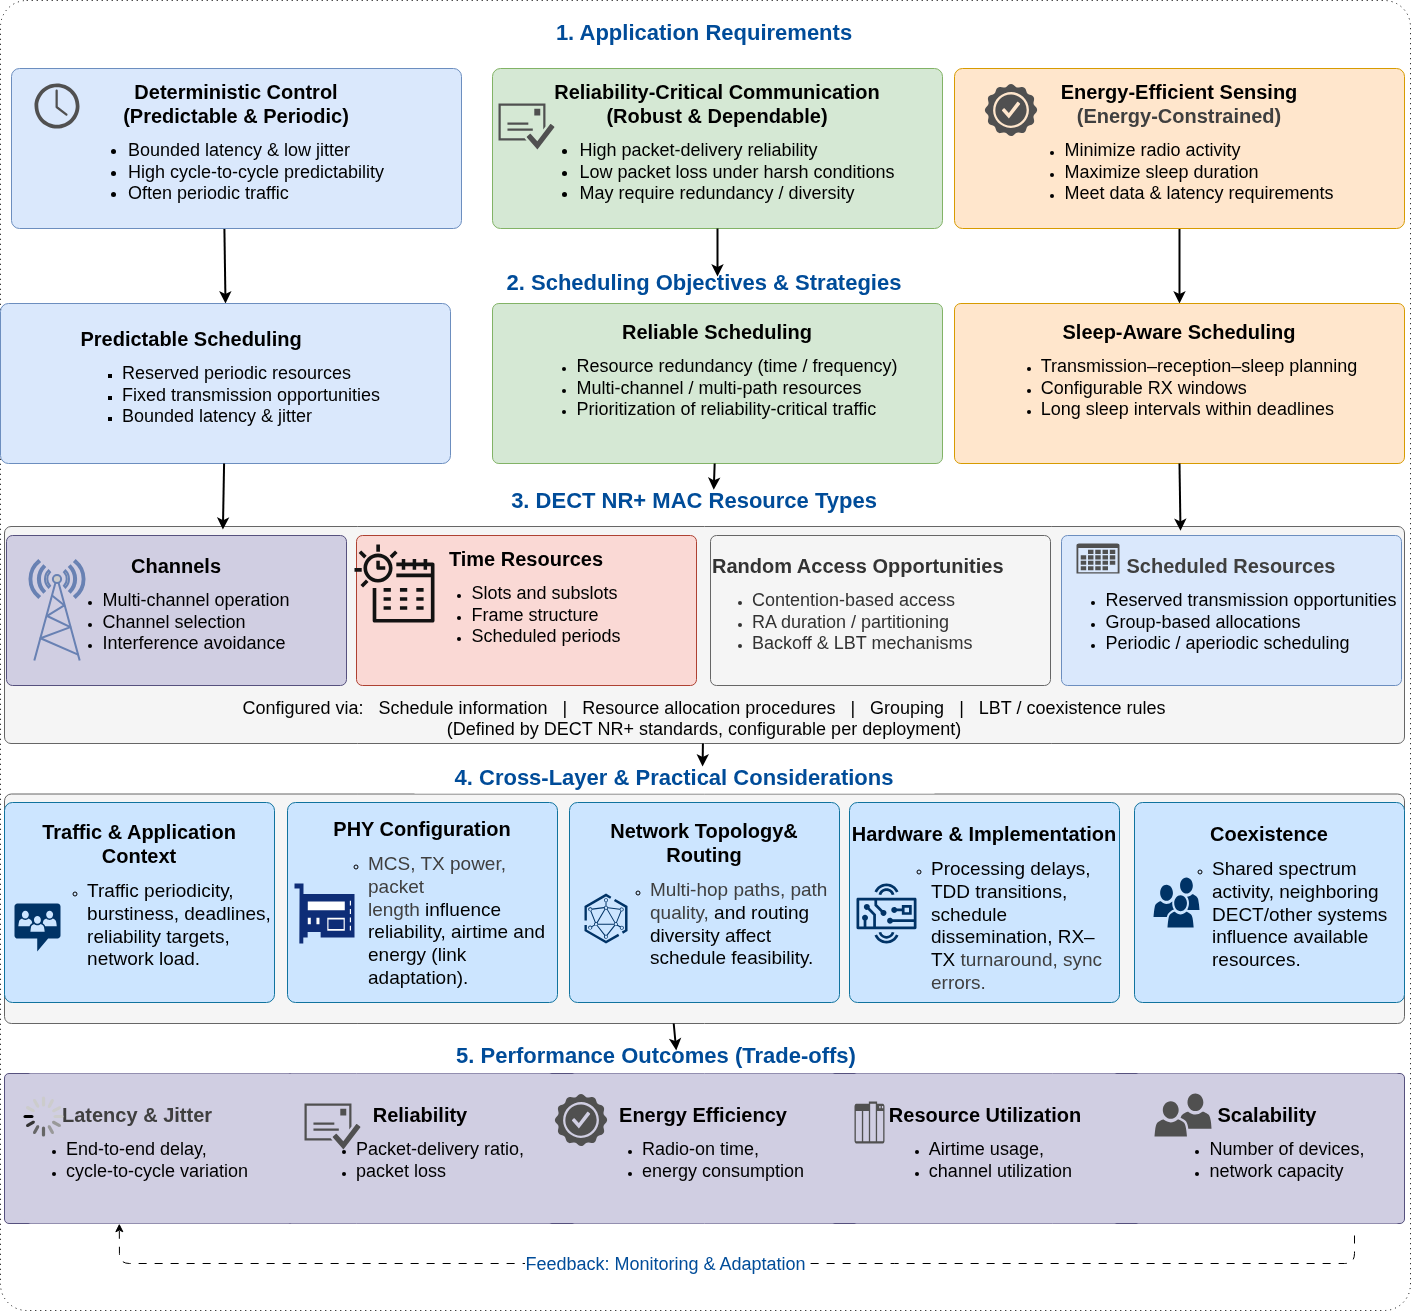
\includegraphics[width=\textwidth]{figures/AppRequirment.png}
    \caption{Application-oriented scheduling and resource-allocation design
    space for DECT NR+. Application requirements motivate different scheduling
    objectives, which are realized through configurable MAC resources and are
    influenced by PHY configuration, network topology, implementation
    constraints, and coexistence conditions. The resulting configurations
    determine trade-offs among latency, reliability, energy efficiency,
    resource utilization, and scalability.}
    \label{fig:application_scheduling}
\end{figure*}

A central scheduling trade-off is the balance between contention-based and scheduled communication. Random access accommodates bursty traffic without permanent resource reservation but becomes less predictable as contention increases, whereas scheduled opportunities improve temporal control at the risk of underutilization. The appropriate balance therefore depends on traffic periodicity, load, device population, and latency requirements \cite{samuylovPerformanceMACLayer2024a, gaidamakaOptimizingDelaysRandom2025}. Gaidamaka et al. illustrate dynamic resource partitioning by using a Hidden Markov Model (HMM) to estimate device activity and adapt the random-access-phase duration. Their numerical results show reduced access delay while preserving more time for data transmission \cite{gaidamakaOptimizingDelaysRandom2025}. However, the approach addresses access-phase allocation rather than the broader problem of distributing scheduled resources among heterogeneous applications.

Latency-sensitive resource configuration is investigated by Glazkov et al., who jointly evaluate LBT, backoff, power control, acknowledgement timing, and priority queuing for near-\gls{urllc} \cite{glazkovImprovingNearURLLCServices2025}. Their simulations report approximately 30--80\% lower multi-hop latency and 10--20\% lower packet loss for the combined configuration, depending on traffic conditions. This indicates that traffic prioritization and transmission timing can materially influence end-to-end performance, although a general scheduler mapping heterogeneous application requirements to resource assignments is not provided.

Resource allocation also interacts with coexistence and PHY configuration. Samuylov et al. show that scheduled access, LBT, and last-minute channel sensing affect spectrum sharing between DECT-2020 NR and classic DECT \cite{samuylovPerformanceAssessmentDECT20202023}. Graf et al., meanwhile, demonstrate experimentally that MCS, transmission power, and packet length produce environment-dependent Pareto-optimal trade-offs among data rate, packet delivery, and energy consumption \cite{grafParetoOptimalityApproach2026a}. Consequently, the value of an allocated transmission opportunity depends not only on its timing but also on the PHY configuration and radio conditions under which it is used.

Comparable application-aware concepts are more mature in cellular resource management. Delay-aware 5G scheduling can incorporate traffic priorities, channel conditions, fairness, and packet delay into resource assignment \cite{madiDelayBasedResourceAllocation2022a}, while programmable RAN frameworks extend traffic control through classification, queueing, scheduling, shaping, and pacing \cite{irazabalTCRANProgrammableTraffic2024}. These approaches cannot be transferred directly because DECT NR+ combines decentralized operation, contention, scheduled resources, flexible FT/PT roles, and native multi-hop communication \cite{etsi_ts103636_1,etsi_ts103636_4}. Nevertheless, they illustrate the broader principle that application and \gls{qos} requirements should influence resource decisions.

This requirement is particularly important in industrial communication, where application periods and deadlines may not align naturally with the radio timing structure. Predictable communication requires coordination among packet generation, resource reservation, schedule repetition, transmission, acknowledgement, and retransmission \cite{etsi_ts103636_3,etsi_ts103636_4}. Reliability may additionally require redundant opportunities or channel diversity, whereas energy-constrained devices benefit from minimizing radio activity and maximizing sleep periods. These objectives create competing demands on the same radio resources \cite{glazkovImprovingNearURLLCServices2025, samuylovEmpoweringNearURLLCIoT2025, grafParetoOptimalityApproach2026a}.

Implementation-level timing further constrains scheduling. Alizai et al. experimentally investigate UL/DL scheduling in DECT-2020 NR star networks using a single-chip DECT NR+ platform, digital-storage-oscilloscope measurements, and internal modem timing analysis \cite{alizaiMeasurementDrivenLatencyAnalysis2026}. The results isolate the RX--TX turnaround associated with alternating reception and transmission and show that, for short-packet and request--response traffic, this turnaround can constitute a significant part of the latency budget. Consequently, reducing the nominal scheduling interval does not necessarily produce a proportional reduction in end-to-end latency on a single-transceiver device. These findings motivate scheduling and architectural approaches that reduce unnecessary UL/DL alternation, including the potential separation of UL and DL resources.

A complementary perspective is provided by analytical queueing studies. Morozova et al. model a DECT-2020 cluster as a discrete-time queue and show that the relative timing of packet generation and service opportunities affects waiting time, sojourn time, and information freshness \cite{morozovaComparisonTwoModels2026a}. Nikolaev et al. extend this perspective using a two-phase tandem queueing model to derive the distribution, mean, and variance of Peak Age of Information (PAoI) \cite{nikolaevModelingDECT2020Tandem2026}. Together, these studies show that resource allocation should consider not only instantaneous access delay and capacity but also traffic generation, queueing, service-time variability, and information freshness.

Overall, existing studies show a progression from static resource configuration toward context-aware management. Random-access duration can be adapted to device activity, MAC parameters and priorities can be coordinated for latency-sensitive traffic, coexistence affects resource availability, PHY configuration changes the utility of allocated resources, and hardware turnaround introduces implementation-level timing constraints. However, these contributions address separate parts of the problem rather than providing a unified application-oriented scheduler. A central open challenge is therefore to map application requirements for latency, reliability, traffic periodicity, and energy to coordinated access, resource, PHY, and timing configurations while accounting for routing and practical hardware constraints.

%%%%%%%%%%%%%%%%%%%%%%%%%%%%%%%%%%%%%%%%%%%%%%%%%%%%%%%%%%%%%%%%%%%%%%%%%%%%%%%%
\subsection{Reliability, URLLC, and mMTC}
\label{subsec:reliability}
%%%%%%%%%%%%%%%%%%%%%%%%%%%%%%%%%%%%%%%%%%%%%%%%%%%%%%%%%%%%%%%%%%%%%%%%%%%%%%%%

Reliability and latency are central objectives in \gls{dectnr} research, particularly because the technology targets demanding \gls{imt2020} use cases while supporting decentralized, large-scale, and multi-hop operation. As shown in Section~\ref{sec:results}, nine of the 51 included studies explicitly address \gls{urllc}, while five address \gls{mmtc}. The literature consistently shows that end-to-end performance emerges from interactions among link quality, channel access, retransmissions, resource configuration, traffic load, routing, topology, and implementation timing \cite{maliatsosEvaluationIMT2020Candidate2022a, smidaETSIDECT2020Component2023, samuylovEmpoweringNearURLLCIoT2025}.

Early studies evaluated whether DECT-2020 NR could satisfy the reliability, latency, and connection-density requirements associated with \gls{urllc} and \gls{mmtc} under the IMT-2020 methodology \cite{maliatsosEvaluationIMT2020Candidate2022a, smidaETSIDECT2020Component2023, pennerURLLCPerformanceEvaluation2021}. These evaluations established a feasibility baseline, while subsequent experimental studies showed that practical reliability depends strongly on radio configuration and environment \cite{haqueDECT2020NRLink2025, bandaraExperimentalValidationAnalysis2025, grafParetoOptimalityApproach2026a}. Modulation and coding, transmission power, packet length, propagation, and interference therefore determine operating points that trade reliability against airtime, throughput, and energy.

The \gls{mmtc} literature exposes similar dependencies at larger scale. Soni et al. evaluate multi-hop decode-and-forward communication and show that outage probability deteriorates with increasing hop count and transmission rate, while coding improves \gls{ber} performance \cite{soniPerformanceMultihopAssisted2021}. Singhwi et al. investigate relay selection, association, and channel allocation in an Urban-Macro scenario and report the most favorable \gls{sinr} distribution for angle-based assignment, with approximately 7~dB difference between the best and worst evaluated approaches \cite{singhwiDECT2020NewRadio2021}. These results demonstrate that massive connectivity depends not only on connection density but also on relay depth, interference, association, and channel allocation.

Combining high reliability with low latency becomes more difficult in multi-hop communication because retransmissions, conservative access, acknowledgements, and forwarding improve delivery probability or reachability while consuming additional time and radio resources \cite{samuylovPerformanceMACLayer2024a, glazkovImprovingNearURLLCServices2025}. Samuylov et al. report approximately 3~ms 95th-percentile latency for direct communication under the evaluated near-\gls{urllc} conditions, whereas multi-hop latency increases to approximately 30~ms \cite{samuylovEmpoweringNearURLLCIoT2025}. This illustrates the substantial latency cost introduced by additional forwarding stages.

Biswas et al. quantify this trade-off for critical-infrastructure monitoring. Their simulations report \gls{harq}-based user-plane latency of approximately 10.55--25.07~ms over five hops and 15.55--38.78~ms over eight hops, depending on packet size \cite{biswasReliableLowLatencyCommunications2024}. Additional retransmissions further increase latency, directly demonstrating that mechanisms intended to recover failed packets consume part of the available latency budget. These values remain scenario-specific because the study considers an optimized, simulation-based mesh under controlled traffic and propagation assumptions.

A complementary recovery strategy is investigated by Mousavi et al., who apply Reed--Solomon (RS) coding as a proactive MAC-layer recovery mechanism for DECT NR+, aiming to reduce dependence on feedback-driven retransmissions \cite{mousaviPerformanceRS2026}. Their design applies RS parity across the Physical Data Channel payloads of grouped slots while leaving synchronization, reference, and control fields outside the RS codeword. The authors evaluate 3-slot packets containing two data slots and one parity slot, 12-slot packets containing nine data slots and three parity slots, and alternative combinations within a common 24-slot radio-frame budget. Using a CRC-aided slot-erasure model, independent Rayleigh fading, and plain ARQ without \gls{harq} soft combining as the baseline, the simulations reveal a reliability--latency--throughput trade-off. Short RS-protected groups localize losses, provide finer recovery granularity, and reduce completion latency under unfavorable channel conditions because recovery can occur without an additional feedback and retransmission cycle. Longer groups amortize repeated PHY signaling and coding overhead more effectively and consequently provide higher useful throughput at moderate-to-high SNR. Mixed frame structures provide an intermediate compromise. The study therefore indicates that RS coding can complement standardized DECT NR+ retransmission mechanisms when bounded recovery time is important; however, the preferred packetization and code configuration remain application- and channel-dependent. These conclusions are limited to the adopted slot-erasure abstraction and plain-ARQ comparison because HARQ soft combining, hardware timing, mobility, interference, and energy consumption were not evaluated.

Glazkov et al. investigate whether coordinated configuration of standardized mechanisms can improve reliability and latency by jointly considering power control, LBT, backoff, priority queuing, and acknowledgement timing \cite{glazkovImprovingNearURLLCServices2025}. Their simulations report approximately 30--80\% lower multi-hop latency and 10--20\% lower packet loss, depending on the \gls{urllc} and \gls{mmtc} traffic conditions, with comparatively limited impact on coexisting \gls{mmtc} traffic. The results show that differentiated traffic treatment and coordinated MAC configuration can improve near-\gls{urllc} performance without replacing the standardized mechanisms.

Routing provides another reliability mechanism because end-to-end performance depends on the quality and number of links traversed. Latency-oriented path selection and topology-aware routing therefore seek to balance reliable links against route length \cite{asifURLLCBasedMultiHopCommunication2025, rauwolfTopologyAwareDeepReinforcement2026a}. Rauwolf et al. explicitly optimize this trade-off using a topology-aware GNN+DRL framework and report reductions of up to 19.9\% in end-to-end latency and 10\% in \gls{per}, together with fewer transmissions relative to the evaluated baselines \cite{rauwolfTopologyAwareDeepReinforcement2026a}. The approach remains simulation-driven, however, leaving computational requirements, online adaptation, and generalization to physical industrial networks open.

Reliability can also be improved by modifying connectivity. Ahmad et al. dynamically assign intermediate FT/PT devices to reconnect nodes in outage regions and report an outage probability below 1\% under the evaluated conditions \cite{ahmadMACProtocolReducing2024}. Subsequent work extends this concept toward ultra-reliable multi-hop \gls{iiot} communication through dynamic intermediate-device assignment and additional MAC/convergence procedures \cite{ahmadMACLayerProtocolUltraReliable2025}. Such topology adaptation can improve connectivity but introduces signaling, forwarding, energy, and route-establishment overhead.

Bin Asif et al. explore a complementary approach by modifying the propagation environment through Intelligent Reflecting Surfaces (IRS) for industrial \gls{urllc} \cite{binasifIRSAssistedDECT2020NR2025}. Their framework identifies shadowed regions and assigns IRS resources together with priority-based subslot allocation. Simulation results report improved received power and throughput and reduced \gls{rtt} relative to the considered conventional and intermediate-node approaches. The approach broadens the reliability design space beyond retransmission and relaying, although IRS control, channel estimation, mobility, synchronization, and hardware integration remain to be experimentally demonstrated.

For \gls{mmtc}, reliability is additionally constrained by contention as device activity increases. Samuylov et al. demonstrate the sensitivity of MAC performance to network density, while Gaidamaka et al. adapt the random-access phase according to estimated device activity \cite{samuylovPerformanceMACLayer2024a, gaidamakaOptimizingDelaysRandom2025}. Together with the relay and link-level studies, the evidence indicates that scalable \gls{mmtc} depends jointly on radio robustness, relay and channel assignment, contention management, and adaptive access.

The coexistence of \gls{urllc} and \gls{mmtc} traffic further requires differentiated resource treatment. Absolute priority for latency-sensitive traffic can disadvantage massive sensing traffic, whereas uniform treatment can prevent \gls{urllc} flows from satisfying deadlines. Existing work shows that traffic priority, access configuration, relay selection, and adaptive resource management can provide such differentiation \cite{samuylovEmpoweringNearURLLCIoT2025, glazkovImprovingNearURLLCServices2025, singhwiDECT2020NewRadio2021}.

Implementation effects become particularly important at tight latency budgets. Measurement-driven UL/DL scheduling analysis shows that RX--TX turnaround on single-transceiver DECT NR+ hardware can constitute a significant component of short-packet and request--response latency \cite{alizaiMeasurementDrivenLatencyAnalysis2026}. Such hardware delays can accumulate with access, forwarding, queueing, acknowledgement, and retransmission delays across multiple hops.

Taken together, the literature identifies several complementary reliability mechanisms: robust PHY configuration, contention and acknowledgement control, retransmission and proactive recovery, resource prioritization, relay assignment, routing, topology adaptation, and propagation enhancement. These mechanisms operate at different layers but affect the same end-to-end objectives and incur different costs in latency, energy, resource utilization, and complexity. The relevant objective is therefore not maximum reliability in isolation, but sufficient reliability within the latency and resource constraints of the application.

Overall, the literature progresses from IMT-2020 feasibility assessment and multi-hop \gls{mmtc} toward cross-layer reliability management involving access, retransmission and recovery, traffic priority, relay assignment, routing, PHY configuration, and propagation enhancement. Nevertheless, much of the multi-hop near-\gls{urllc} and massive-\gls{mmtc} evidence remains analytical or simulation-based. Experimental studies have validated important link, commercial-device, and implementation-timing characteristics \cite{haqueDECT2020NRLink2025, bandaraExperimentalValidationAnalysis2025, grafParetoOptimalityApproach2026a, alizaiMeasurementDrivenLatencyAnalysis2026}, but comparable large-scale end-to-end reliability experiments remain limited. This motivates application-oriented evaluation under realistic interference, heterogeneous traffic, mobility, failures, variable device activity, and hardware timing, with reliability assessed jointly with latency, energy, and resource cost.


%%%%%%%%%%%%%%%%%%%%%%%%%%%%%%%%%%%%%%%%%%%%%%%%%%%%%%%%%%%%%%%%%%%%%%%%%%%%%%%%
\subsection{Energy Efficiency}
\label{subsec:energy}
%%%%%%%%%%%%%%%%%%%%%%%%%%%%%%%%%%%%%%%%%%%%%%%%%%%%%%%%%%%%%%%%%%%%%%%%%%%%%%%%

Energy efficiency is an important objective for \gls{dectnr}, particularly for battery-powered sensing and \gls{mmtc} applications. As shown in Section~\ref{sec:results}, eight of the 51 included studies address energy-related aspects. The literature shows that communication energy depends not only on transmission power but also on radio duty cycle, reception, forwarding, topology, PHY configuration, retransmissions, traffic, and latency requirements.

At the network level, Kovalchukov et al. show that multi-hop communication can reduce transmission energy relative to direct long-range links under the evaluated \gls{mmtc} conditions \cite{kovalchukovDECT2020NewRadio2022}. However, increasing routing bias and hop count also increases forwarding energy, with device density and interference influencing the resulting balance. Multi-hop operation therefore does not provide an unconditional energy advantage; its benefit depends on the trade-off between shorter transmission distances and additional forwarding activity.

Nihtila and Berg examine this trade-off from the perspective of battery-powered mesh operation and identify a fundamental tension between communication latency and device lifetime \cite{nihtilaEnergyConsumptionDECT20202022}. Leaf devices carrying sporadic traffic can remain inactive for comparatively long periods, whereas forwarding nodes must provide sufficiently frequent receive opportunities. Shorter availability intervals reduce forwarding latency but increase radio-on time, creating asymmetric energy consumption between leaf and router devices.

To distribute this forwarding burden, Nihtila and Taipale propose periodic router rotation among eligible nodes \cite{nihtilaEnergySavingRouter2022}. Their simulations show that rotating forwarding responsibility can improve the distribution of energy consumption and extend network lifetime relative to static router assignment. This distinguishes device-level energy efficiency from network lifetime: minimizing aggregate communication energy does not necessarily prevent strategically important forwarding nodes from being depleted prematurely. Energy-aware routing must therefore consider both communication performance and the distribution of forwarding cost across devices \cite{nihtilaEnergyConsumptionDECT20202022, nihtilaEnergySavingRouter2022}.

Experimental work complements these system-level studies with measurements on commercial DECT NR+ hardware. Bandara reports energy costs of approximately 0.26--2.6~$\mu$J/bit depending on MCS and operating conditions, together with measurements of range, throughput, and latency \cite{bandaraExperimentalValidationAnalysis2025}. The approximately order-of-magnitude variation indicates that PHY configuration strongly affects the energy required to deliver useful information and that energy metrics should be interpreted together with delivery reliability and application requirements.

Graf et al. further show that modem current consumption differs substantially across radio states and increases at high transmission power \cite{grafWhatExpectWhen2026}. Their subsequent multi-objective analysis jointly considers MCS, transmit power, packet length, data rate, PDR, and energy consumption and identifies environment-dependent Pareto-optimal configurations \cite{grafParetoOptimalityApproach2026a}. Lower transmit power does not necessarily minimize energy if it increases packet errors and retransmissions, while robust configurations may increase airtime. Energy-efficient PHY operation is therefore application- and channel-dependent rather than represented by a universally optimal radio configuration.

These results connect energy directly to scheduling and reliability. Applications with relaxed reporting deadlines can tolerate longer inactive periods, whereas latency-sensitive communication requires more frequent radio availability. Similarly, deteriorating channels or stringent reliability requirements can require increased transmission power, robust modulation, or retransmissions, each increasing energy consumption. Energy optimization must therefore consider radio configuration, activity scheduling, and communication requirements jointly \cite{nihtilaEnergyConsumptionDECT20202022, bandaraExperimentalValidationAnalysis2025, grafParetoOptimalityApproach2026a}.

A substantially different operating regime is introduced by ambient backscatter. Liao et al. investigate whether existing DECT NR+ transmissions can serve as an ambient RF source for extremely low-power devices \cite{liaoDataAssistedBackscatter2025}. Their design integrates a backscatter receiver with a DECT NR+ SDR receiver and exploits waveform structure for data-assisted detection. Over-the-air experiments demonstrate feasibility, with \gls{ber} values as low as 0.02 under the most favorable evaluated conditions. Although still a proof of concept, this approach broadens the energy design space beyond optimization of active radios and could support sensing devices with substantially smaller power budgets. Practical challenges remain in range, multi-device access, synchronization, scheduling, interference, and operation in industrial channels.

The reviewed evidence can therefore be interpreted at three interacting levels. At the device and link level, modem state, MCS, transmission power, packet length, and delivery probability determine communication energy \cite{bandaraExperimentalValidationAnalysis2025, grafWhatExpectWhen2026, grafParetoOptimalityApproach2026a}. At the network level, transmission distance, topology, hop count, router availability, and forwarding responsibility determine both aggregate consumption and its distribution across devices \cite{kovalchukovDECT2020NewRadio2022, nihtilaEnergyConsumptionDECT20202022, nihtilaEnergySavingRouter2022}. At the system level, ambient backscatter extends DECT NR+-based communication toward devices with substantially lower power budgets \cite{liaoDataAssistedBackscatter2025}.

These findings are consistent with broader energy-efficient wireless MAC research, where reducing idle listening, unnecessary reception, contention, overhearing, and radio-on time is fundamental \cite{tsaoSurveyEnergyEfficient2011}. DECT NR+ adds the complication that native multi-hop operation makes a device's sleep schedule dependent not only on its own traffic but also on its forwarding responsibility. Sleep-aware scheduling, energy-aware routing, and router-role assignment are consequently closely coupled \cite{nihtilaEnergyConsumptionDECT20202022, nihtilaEnergySavingRouter2022}.

Overall, the literature indicates that DECT NR+ energy efficiency is a cross-layer property. Transmission parameters determine link-level energy; topology and routing distribute forwarding costs; duty cycle determines background reception energy; scheduling determines radio availability; and reliability requirements introduce additional airtime or retransmissions. However, mesh-level energy and router-role studies remain predominantly simulation-based, whereas detailed hardware measurements mainly characterize point-to-point operation \cite{nihtilaEnergyConsumptionDECT20202022, nihtilaEnergySavingRouter2022, bandaraExperimentalValidationAnalysis2025, grafWhatExpectWhen2026, grafParetoOptimalityApproach2026a}. A major remaining challenge is therefore experimentally validated, application-oriented lifetime optimization that jointly considers sleep-aware scheduling, residual-energy-aware relay selection, router rotation, adaptive PHY configuration, application deadlines, and battery state.


%%%%%%%%%%%%%%%%%%%%%%%%%%%%%%%%%%%%%%%%%%%%%%%%%%%%%%%%%%%%%%%%%%%%%%%%%%%%%%%%
\subsection{Positioning and Localization}
\label{subsec:positioning}
%%%%%%%%%%%%%%%%%%%%%%%%%%%%%%%%%%%%%%%%%%%%%%%%%%%%%%%%%%%%%%%%%%%%%%%%%%%%%%%%

Positioning and localization represent an emerging research direction within
\gls{dectnr}. As shown in Section~\ref{sec:results}, six of the 51 included studies address positioning or localization, while only two are classified primarily in this category. Compared with PHY, MAC, and routing, localization is therefore comparatively less developed in the reviewed literature. A central challenge is to obtain useful positioning information without excessive measurement, signaling, processing, and energy overhead \cite{saikkoPositioningDECT2020NR2024, saikkoPositioningTrackingDECT20202025}.

Saikko et al. address this problem through proactive measurement selection using time-of-arrival-based range and angle-of-arrival measurements \cite{saikkoPositioningDECT2020NR2024}. Rather than acquiring measurements from all available anchors, Fisher information is used together with prior state information from an extended Kalman filter (EKF) to select measurements expected to contribute most strongly to positioning accuracy. This differs from SNR-based selection because a high-quality measurement may provide little additional geometric information when it is redundant with existing observations.

The numerical results show substantial benefits when only a limited number of anchors is selected. With two range-measurement anchors, positioning RMSE is approximately 47.5--62.5\% lower than with the SNR-based reference, while three selected anchors provide approximately 20.1--31.4\% lower RMSE \cite{saikkoPositioningDECT2020NR2024}. Tail performance also improves substantially: with two range anchors and a 1~s measurement interval, the 99.9th-percentile positioning error is approximately 0.84~m compared with 6.13~m for SNR-based selection \cite{saikkoPositioningDECT2020NR2024}. These results indicate that positioning accuracy can be improved without indiscriminately increasing the number of measurements.

Saikko et al. subsequently extend the framework toward multimodal positioning and tracking using range, angle, and received signal strength (RSS) measurements together with EKF- and particle-filter-based tracking \cite{saikkoPositioningTrackingDECT20202025}. Fisher-information-based selection again prioritizes measurements according to their expected contribution. With two selected anchors, the reported positioning RMSE is approximately 10--50\% lower than with SNR-based selection, depending on measurement type and conditions, while reductions in the largest positioning errors reach approximately 60\% \cite{saikkoPositioningTrackingDECT20202025}. The study also shows that selection performance depends on the quality of prior state information; longer measurement intervals and increased prediction uncertainty can reduce the reliability of anchor selection.

Together, these studies establish an important principle for DECT NR+ localization: positioning should optimize the \emph{information value} of measurements rather than simply maximizing the number acquired. Measurement selection consequently becomes a resource-management problem because fewer, more informative measurements can reduce signaling, processing, radio activity, and potentially energy consumption while maintaining positioning performance.

Localization can also support network operation. F{\"u}hrling et al. incorporate multi-hop localization into a routing framework for partially known mesh topologies, using estimated relative node positions to support local route discovery \cite{fuhrlingRobustRoutingProtocol2025b}. This illustrates two complementary roles for localization in DECT NR+: \emph{application-level positioning}, in which location is the required service, and \emph{network-assisted localization}, in which spatial information supports functions such as routing or topology management.

The available evidence nevertheless remains predominantly analytical and simulation-based \cite{saikkoPositioningDECT2020NR2024, saikkoPositioningTrackingDECT20202025}. Comparable large-scale localization measurements on commercial DECT NR+ hardware in industrial environments remain limited. This is important because NLoS propagation, metallic structures, dynamic blockage, multipath, synchronization, antenna geometry, and mobility can introduce measurement errors that are difficult to represent completely through idealized models.

Positioning also interacts directly with communication resources. Increasing measurement frequency or the number of participating anchors can improve tracking information but consumes additional radio, processing, and energy resources, whereas sparse measurements reduce overhead at the cost of greater state uncertainty \cite{saikkoPositioningDECT2020NR2024, saikkoPositioningTrackingDECT20202025}. Localization should therefore ultimately be treated as a joint communication--positioning resource-management problem involving measurement modality, anchor selection, update interval, mobility, state uncertainty, and application accuracy requirements.

Native multi-hop operation additionally creates opportunities for cooperative localization. The use of multi-hop localization for routing already provides an initial indication of this potential \cite{fuhrlingRobustRoutingProtocol2025b}, but cooperative accuracy, signaling overhead, synchronization, error propagation, and scalability remain largely unexplored.

Overall, DECT NR+ positioning research has progressed from proactive selection of range and angle measurements toward multimodal range--angle--RSS tracking. Information-aware measurement selection can substantially improve positioning performance when measurement resources are limited. However, experimental maturity remains below that of communication-oriented DECT NR+ research, particularly for hardware-based industrial localization, mobility and NLoS conditions, multimodal fusion, adaptive measurement intervals, cooperative mesh positioning, and integration of positioning with MAC scheduling and energy management.


%%%%%%%%%%%%%%%%%%%%%%%%%%%%%%%%%%%%%%%%%%%%%%%%%%%%%%%%%%%%%%%%%%%%%%%%%%%%%%%%
\subsection{Security, Coexistence, and Multi-RAT Integration}
\label{subsec:security_coexistence}
%%%%%%%%%%%%%%%%%%%%%%%%%%%%%%%%%%%%%%%%%%%%%%%%%%%%%%%%%%%%%%%%%%%%%%%%%%%%%%%%

Security, coexistence, and heterogeneous-network integration remain comparatively underexplored in the \gls{dectnr} literature. As shown in Section~\ref{sec:results}, only three of the 51 included studies were coded under security or multi-RAT integration, while two explicitly address coexistence or regulatory aspects. Compared with PHY, MAC, and routing, these deployment-oriented topics are therefore comparatively less developed in the reviewed literature.

The available evidence can be synthesized across three interacting deployment dimensions. Security determines trusted participation and communication protection \cite{etsi_ts103636_4,etsi_ts103636_5}; coexistence determines how DECT NR+ shares spectrum under technical and regulatory constraints \cite{samuylovPerformanceAssessmentDECT20202023, samuylovPerformanceDECT2020NR2025}; and multi-RAT integration determines how DECT NR+ cooperates with complementary radio and core-network technologies \cite{dangEWDCIntegratingDECT20202025a, dangUniRATUnifiedDECT20202026}. These dimensions are coupled because interference can trigger channel or RAT changes, inter-RAT transitions can require security procedures, and authentication and tunneling introduce processing and signaling overhead.

Security functionality is integral to the standardized DECT NR+ architecture. The specifications define mechanisms for device identification, authentication, key management, integrity protection, and confidentiality \cite{etsi_ts103636_4,etsi_ts103636_5}. In multi-hop networks, however, security extends beyond individual radio links because devices can participate in forwarding, topology formation, relay selection, and dynamic FT/PT relationships. Increasingly sophisticated routing mechanisms based on topology and link information consequently depend on the trustworthiness of distributed network state \cite{fuhrlingRobustRoutingProtocol2025b, rauwolfTopologyAwareDeepReinforcement2026a}.

Comparable threats are well established in other low-power mesh networks, where manipulation of routing information has motivated lightweight detection mechanisms for attacks such as rank manipulation \cite{kalyaniResourceefficientEnsembleMachine2026}. This evidence is used only for contextual comparison rather than as evidence about DECT NR+ itself. Nevertheless, it illustrates relevant questions for future DECT NR+ evaluation, including routing manipulation, falsified topology information, unauthorized participation, and resource-exhaustion attacks.

For additional contextual evidence beyond the 51-study primary corpus, Ngo addresses security from an interworking perspective by integrating resource-constrained non-cellular IoT devices, including DECT-2020 NR platforms, with 5G-core authentication and session management \cite{ngoIoTDeviceAuthentication2025}. The architecture transfers substantial authentication and traffic-control functionality toward the 5G core rather than requiring a complete cellular security stack on every constrained device, and interoperability is demonstrated with commercial and open-source 5G core platforms. Although this work is not part of the quantitative primary corpus, it provides a relevant pathway for incorporating DECT NR+-based devices into broader infrastructure-managed security architectures.

A second deployment challenge is spectrum coexistence. DECT NR+ channel access depends on sensing, LBT, backoff, and resource-selection procedures, which influence both internal performance and interaction with other spectrum users \cite{etsi_ts103636_2,etsi_ts103636_4}. Samuylov et al. evaluate coexistence between DECT-2020 NR and classic DECT using LBT, last-minute scanning, and scheduling-based mechanisms \cite{samuylovPerformanceAssessmentDECT20202023}. Under the evaluated conditions, standard LBT keeps classic-DECT packet drops below approximately 2\% when 25\% of resources are allocated to classic DECT. Last-minute scanning increases DECT-2020 NR packet drops by more than 10\% relative to LBT-only operation, whereas the considered scheduling approach improves DECT-2020 NR performance by approximately 2--5\%. These results indicate that coexistence performance depends on the particular sensing and scheduling strategy rather than channel occupancy alone.

Regulatory access rules can impose additional constraints. Samuylov et al. compare native DECT-2020 NR LBT with mesh operation following FCC access rules for the UPCS band \cite{samuylovPerformanceDECT2020NR2025}. In the evaluated scenarios, packet delivery for the FCC-based mesh falls below 85\%, compared with approximately 98--99\% using native DECT NR+ LBT, while the effect on coexisting classic-DECT devices remains comparatively small. The result shows that practical mesh performance depends not only on the radio protocol but also on the regulatory spectrum-access regime.

A third direction concerns deliberate cooperation between DECT NR+ and other \glspl{rit}. Rather than using one technology for every function, heterogeneous architectures can exploit complementary capabilities: DECT NR+ for decentralized discovery and direct or multi-hop communication, Wi-Fi for high-throughput local transfer, and 5G infrastructure for authentication, session management, and external connectivity.

Dang et al. demonstrate this principle through enhanced wireless direct connectivity (EWDC), which combines DECT-2020 NR and Wi-Fi \cite{dangEWDCIntegratingDECT20202025a}. DECT is used for discovery and secure exchange of Wi-Fi configuration information, while Wi-Fi carries the high-bandwidth data path. The implementation uses Nordic nRF9161-DK hardware, with WireGuard protecting Wi-Fi communication. EWDC therefore illustrates a functional division between control/discovery and data transmission rather than requiring both radios to carry identical traffic.

The subsequent Uni-RAT framework extends this concept to DECT-2020 NR, Wi-Fi, and a 5G core \cite{dangUniRATUnifiedDECT20202026}. DECT-2020 NR operates as the Master-RAT and anchors control-plane security through 5G-AKA and NAS, while Wi-Fi acts as a Secondary-RAT for data delivery. WireGuard protects Layer-3 communication, and customized NAS signaling distributes configuration and keying information. A physical prototype combines Nordic nRF9161 DECT devices, Raspberry Pi Wi-Fi nodes, a commercial 5G core, and Arm TrustZone for security-critical functionality.

Taken together, the interworking studies indicate a progression toward functional and security integration across DECT NR+, Wi-Fi, and 5G infrastructure \cite{dangEWDCIntegratingDECT20202025a, dangUniRATUnifiedDECT20202026}. Such integration expands the trust boundary across radio interfaces, gateways, security contexts, configuration exchange, and core-network functions. Multi-RAT systems must additionally decide which interface should carry a traffic flow and when another RAT should be activated according to application requirements and radio conditions.

Despite recent progress, experimental evidence remains limited. Coexistence studies are predominantly simulation-based \cite{samuylovPerformanceAssessmentDECT20202023, samuylovPerformanceDECT2020NR2025}, whereas the available multi-RAT prototypes cover only a subset of possible authentication, mobility, failover, routing, and heterogeneous-traffic scenarios \cite{dangEWDCIntegratingDECT20202025a, dangUniRATUnifiedDECT20202026}. Security of native multi-hop operation is a particularly important gap because increasingly sophisticated routing and topology-management mechanisms have not yet been matched by comparable attack-oriented experimental analysis.

Overall, the evidence shows a progression from standardized security and autonomous spectrum access toward heterogeneous connectivity architectures. Coexistence and regulatory constraints can materially affect packet-delivery performance, while EWDC and Uni-RAT demonstrate practical pathways for integrating DECT NR+ with Wi-Fi and 5G infrastructure. Important remaining questions concern secure multi-hop operation, attack-oriented evaluation, interference-aware channel selection, application-aware RAT selection, mobility and failover, and experimental characterization of the latency, energy, and signaling overhead introduced by security and interworking mechanisms.


%%%%%%%%%%%%%%%%%%%%%%%%%%%%%%%%%%%%%%%%%%%%%%%%%%%%%%%%%%%%%%%%%%%%%%%%%%%%%%%%
\subsection{Industrial Applications and Experimental Implementations}
\label{subsec:industrial_experimental}
%%%%%%%%%%%%%%%%%%%%%%%%%%%%%%%%%%%%%%%%%%%%%%%%%%%%%%%%%%%%%%%%%%%%%%%%%%%%%%%%

Experimental and application-oriented research provides an important measure of the technological maturity of \gls{dectnr}. As shown in Section~\ref{sec:results}, 14 of the 51 included studies have an industrial or application-oriented primary contribution, while 18 address experimental, testbed, or application aspects. Across the corpus, 16 studies employ hardware prototypes, 11 use commercial devices, five report field-trial activities, and three include measurements in industrial environments. The literature has therefore progressed beyond standardization and simulation, although the scale and realism of experimental validation vary considerably.

Industrial propagation measurements provide one important source of empirical evidence. Wa{\ss}mann et al. investigate DECT-2020 NR at 450, 1350, and 3700~MHz using MATLAB/GNU Radio and USRP B210 hardware and report an average RMS delay spread of approximately 65~ns for the 13.824~MHz configuration \cite{wassmannPerformanceDECT2020NR2024}. Haque et al. complement these measurements with practical range evaluation, demonstrating packet-success rates above 90\% for indoor NLoS communication beyond 60~m at 0~dBm and outdoor LoS communication beyond 600~m at 19~dBm \cite{haqueDECT2020NRLink2025}. Together, these studies demonstrate substantial coverage potential while confirming the strong dependence of practical performance on propagation conditions and radio configuration.

Commercial-device experiments broaden this evidence to multiple \glspl{kpi}. Bandara evaluates Nordic nRF91-series hardware and reports outdoor LoS communication of approximately 730~m at an 80\% packet-delivery ratio, maximum measured throughput of approximately 2.50~Mbit/s for MCS~4 with eight subslots compared with approximately 3.36~Mbit/s theoretically, and a minimum measured \gls{rtt} of approximately 2.255~ms for a 12-byte payload \cite{bandaraExperimentalValidationAnalysis2025}. Energy consumption varies from approximately 0.26 to 2.6~$\mu$J/bit depending on configuration, illustrating that range, throughput, latency, reliability, and energy must be interpreted jointly.

Graf et al. similarly characterize practical radio behavior and power consumption on commercial DECT NR+ hardware \cite{grafWhatExpectWhen2026}. Their subsequent measurement-driven multi-objective analysis evaluates MCS, transmit power, and packet length and identifies environment-dependent Pareto-optimal configurations across data rate, packet delivery, and energy consumption \cite{grafParetoOptimalityApproach2026a}. These studies represent a transition from hardware characterization toward experimentally informed configuration according to application requirements.

Application-oriented prototypes provide a further level of validation. Mudriievskyi et al. construct a low-cost DECT NR+ testbed for Tactile Internet and human-in-the-loop communication using commercial platforms \cite{mudriievskyiCHEAP5GDECT2024a}. Their non-optimized COTS implementation achieves approximately 2--8~ms latency and 2.3--2.5~Mbit/s under the evaluated packet lengths and MCS configurations. Although limited to two platforms and primarily point-to-point communication, the experiment demonstrates practical low-latency operation on comparatively inexpensive hardware.

Professional live audio constitutes another application domain with stringent latency and reliability requirements. D{\"u}rre and Werner explore the DECT-2020 NR design space for professional live audio using Nordic nRF91-series modem hardware and practical latency measurements \cite{durreDECT2020NRProfessional2024}. Their evaluation considers the trade-off among latency, RF-resource utilization, and transmission robustness and identifies a minimum measured latency of approximately 2.312~ms with the available modem implementation, at the cost of roughly one third of the RF channel resources. Because the implementation available for the study primarily exposed PHY-level functionality, the reported value should be interpreted as a minimum implementation-latency estimate rather than a complete application-level audio delay.

Poets and Wa{\ss}mann subsequently broaden the professional-audio perspective by examining the DECT NR+ design space for wireless microphones and media applications \cite{poetsDECTNRNew2024}. Later work implements a functional prototype connecting two Dante-enabled audio devices through an open-source DECT NR+ SDR implementation \cite{poetsProfessionalNetworkedAudio2025}. The prototype achieves an average one-way latency of approximately 1.7~ms. Unlike isolated PHY or packet measurements, this application-level demonstration additionally exposes synchronization, periodic traffic, buffering, and application-specific \gls{qos} requirements. Taken together, the professional-audio studies show a progression from radio-level design-space exploration and modem-latency measurement toward end-to-end application prototyping.

Power-grid monitoring extends experimental validation toward multi-hop and heterogeneous application traffic. Pires et al. evaluate DECT-2020 NR mesh networking for temperature and humidity monitoring, video-based intrusion detection, and power-quality monitoring \cite{piresDECT2020NREnergy2026b}. Under two-hop conditions, the three substation use cases exhibit mean mesh latencies of approximately 15.45, 18.55, and 27.93~ms and corresponding end-to-end mean latencies of approximately 26.6, 29.71, and 39.62~ms. The difference illustrates the additional delay introduced by gateway and backhaul components beyond the DECT NR+ mesh itself. A second proof of concept uses five nRF9151/nRF9161-based nodes in a four-hop mesh and includes a 48-hour power-quality measurement experiment, providing evidence beyond short-duration point-to-point testing.

The application landscape also extends beyond fixed industrial and indoor deployments. Jahangir investigates DECT NR+ connectivity for unmanned aerial vehicles through analytical link-budget modeling and simulation of air-to-ground and air-to-air communication \cite{jahangirAnalysisPerformanceDECT2024}. The analysis considers frequencies of 915~MHz, 1.89~GHz, and 3.5~GHz together with different modulation schemes and communication distances. Under the modeled conditions, lower-frequency operation, particularly at 915~MHz, provides more favorable long-range link behavior because of reduced path loss, whereas the higher-frequency options become increasingly constrained as distance grows. The study broadens the potential application space of DECT NR+ toward aerial connectivity, but its evidence remains analytical and simulation-based; UAV flight tests, mobility, altitude-dependent propagation, antenna orientation, Doppler effects, and dynamic routing remain open for experimental validation.

Implementation-oriented research also addresses the realization of individual PHY functions. Fagerholm et al. propose an FPGA-oriented synchronization architecture requiring only two complex multiplications \cite{fagerholmFPGAbasedDECT2020New2024}. Evaluation with MATLAB, Icarus Verilog, and captured real-world data indicates an additional \gls{snr} requirement of approximately 2.6~dB or more depending on configuration. The work demonstrates efficient hardware-oriented synchronization, although it should not be interpreted as a complete FPGA-based DECT NR+ PHY/MAC testbed.

Recent measurement-driven work extends experimentation toward internal scheduling behavior. Alizai et al. investigate UL/DL scheduling on a single-chip DECT NR+ platform using digital-storage-oscilloscope measurements and internal modem timing analysis \cite{alizaiMeasurementDrivenLatencyAnalysis2026}. By isolating the RX--TX turnaround associated with alternating reception and transmission, the study shows that hardware switching can constitute a significant component of the latency budget for short-packet and request--response communication. Consequently, reducing nominal scheduling delay alone does not necessarily produce a proportional reduction in application-visible latency on single-transceiver hardware, motivating scheduling and architectural approaches that reduce unnecessary UL/DL alternation.

The experimental literature therefore spans complementary implementation platforms. Commercial Nordic nRF91-series devices provide standardized modem realism \cite{durreDECT2020NRProfessional2024, bandaraExperimentalValidationAnalysis2025, grafWhatExpectWhen2026, mudriievskyiCHEAP5GDECT2024a, piresDECT2020NREnergy2026b}; SDR platforms provide greater PHY and application-level flexibility \cite{wassmannPerformanceDECT2020NR2024, poetsProfessionalNetworkedAudio2025}; and FPGA-oriented work provides architectural control over digital implementation \cite{fagerholmFPGAbasedDECT2020New2024}. These approaches collectively show a progression from radio characterization toward measurement-driven configuration and application-level validation. The UAV analysis complements these hardware studies by illustrating how analytical modeling can be used to explore application domains that have not yet reached physical deployment \cite{jahangirAnalysisPerformanceDECT2024}.

Across application domains, different studies expose different aspects of DECT NR+. Tactile communication emphasizes short-packet latency; professional audio adds stringent periodic traffic, synchronization, and RF-resource constraints; power-grid monitoring introduces heterogeneous traffic, gateways, multi-hop communication, and longer-duration operation; UAV analysis introduces mobility-oriented range and frequency considerations; industrial measurements expose realistic propagation; and device-level studies reveal implementation and energy constraints. Application suitability should therefore be established through use-case-specific requirements rather than a generic claim of industrial applicability.

Despite this progress, experimental maturity remains uneven. Many hardware studies involve small device populations, static topologies, limited traffic diversity, or controlled radio conditions. Moreover, differences in MCS, transmit power, payload, topology, hop count, offered load, interference, and measurement duration make direct comparison difficult. Some application domains, such as UAV connectivity, remain primarily model-based rather than experimentally demonstrated \cite{jahangirAnalysisPerformanceDECT2024}. Reproducible benchmark scenarios and clearly defined measurement boundaries are therefore needed, particularly because gateway, backhaul, transport, and application processing can contribute substantially to end-to-end latency \cite{piresDECT2020NREnergy2026b}.

Overall, DECT NR+ research has progressed from conceptual and simulation-based feasibility toward industrial-channel measurements, commercial-device characterization, SDR implementations, application prototypes, multi-hop proofs of concept, and implementation-level timing analysis. The central experimental question is consequently shifting from whether DECT NR+ can operate to how its PHY, MAC, scheduling, routing, topology, and hardware configuration should be selected for specific applications. Larger and more representative physical deployments are still required to evaluate multi-hop communication, mobility, heterogeneous traffic, interference, failures, multi-channel operation, and long-duration behavior while jointly relating latency distributions, jitter, reliability, throughput, energy, and network lifetime to application requirements.
%%%%%%%%%%%%%%%%%%%%%%%%%%%%%%%%%%%%%%%%%%%%%%%%%%%%%%%%%%%%%%%%%%%%%%%%%%%%%%%%
\section{Discussion and Research Gaps}
\label{sec:discussion}
%%%%%%%%%%%%%%%%%%%%%%%%%%%%%%%%%%%%%%%%%%%%%%%%%%%%%%%%%%%%%%%%%%%%%%%%%%%%%%%%

The results of this systematic review show that research on \gls{dectnr} has expanded rapidly since its introduction within the \gls{imt2020} standardization process. The literature now spans PHY and MAC operation, multi-hop networking, reliability, resource management, energy efficiency, positioning, coexistence, and application-oriented implementations. However, the evidence is unevenly distributed across these areas and remains heterogeneous in both methodology and experimental scale. This section interprets the quantitative and technical findings of the review, identifies the principal limitations of the current evidence base, and derives research priorities for further investigation of DECT NR+ in industrial wireless systems.


%%%%%%%%%%%%%%%%%%%%%%%%%%%%%%%%%%%%%%%%%%%%%%%%%%%%%%%%%%%%%%%%%%%%%%%%%%%%%%%%
\subsection{Maturity of the DECT-2020 NR Research Landscape}
\label{subsec:research_maturity}
%%%%%%%%%%%%%%%%%%%%%%%%%%%%%%%%%%%%%%%%%%%%%%%%%%%%%%%%%%%%%%%%%%%%%%%%%%%%%%%%

The publication trend indicates a rapidly expanding but still comparatively young research field. Approximately 75\% of the 51 included studies were published between 2024 and July 2026, and 36 studies appeared as conference publications. This concentration of recent work indicates continued exploration of fundamental mechanisms, implementation strategies, and application opportunities rather than convergence toward widely established and extensively validated design practices.

Research maturity also differs substantially across technical areas. PHY, MAC, and routing/mesh networking are the most frequently investigated topics, with 22, 22, and 23 studies addressing these areas, respectively. Experimental, testbed, or application-related aspects appear in 18 studies, indicating an increasing transition from analytical and simulation-based feasibility studies toward physical implementation. In contrast, scheduling and resource allocation, positioning, security, coexistence, and multi-RAT integration remain less extensively investigated. The reviewed evidence is therefore strongest for fundamental communication mechanisms and more limited for several functions that become increasingly important when DECT NR+ is deployed as part of a complete industrial communication system.

The methodological distribution reinforces this interpretation. Simulation is used in 32 studies and analytical or modeling approaches in 23, whereas 16 studies employ experimental or testbed evaluation. Hardware-based investigations are particularly important because they expose implementation effects that are difficult to represent completely in abstract models, including industrial propagation, modem energy consumption, implementation-dependent throughput, gateway processing, and RX--TX turnaround behavior \cite{wassmannPerformanceDECT2020NR2024, bandaraExperimentalValidationAnalysis2025, grafWhatExpectWhen2026, piresDECT2020NREnergy2026b, alizaiMeasurementDrivenLatencyAnalysis2026}. The literature has therefore progressed beyond exclusively analytical and simulation-based evaluation, but the degree of experimental validation remains uneven across research areas.


%%%%%%%%%%%%%%%%%%%%%%%%%%%%%%%%%%%%%%%%%%%%%%%%%%%%%%%%%%%%%%%%%%%%%%%%%%%%%%%% \subsection{Cross-Layer and Application-Oriented Design}
\label{subsec:cross_layer_gaps}
%%%%%%%%%%%%%%%%%%%%%%%%%%%%%%%%%%%%%%%%%%%%%%%%%%%%%%%%%%%%%%%%%%%%%%%%%%%%%%%%

One of the clearest conclusions of the technical synthesis is that DECT NR+ performance is inherently cross-layer. PHY configuration affects data rate, coverage, reliability, airtime, and energy consumption \cite{grafParetoOptimalityApproach2026a}; MAC and channel-access mechanisms influence contention and access delay \cite{samuylovPerformanceMACLayer2024a, gaidamakaOptimizingDelaysRandom2025}; and routing decisions affect hop count, forwarding load, latency, and reliability \cite{asifURLLCBasedMultiHopCommunication2025, alamDLRoutingPerformance2026a, rauwolfTopologyAwareDeepReinforcement2026a}. Network lifetime is additionally affected by router availability and role assignment \cite{nihtilaEnergyConsumptionDECT20202022, nihtilaEnergySavingRouter2022}, while hardware constraints can alter the latency achievable by otherwise efficient schedules \cite{alizaiMeasurementDrivenLatencyAnalysis2026}.

Fig.~\ref{fig:cross_layer_framework} summarizes these dependencies from an application-oriented perspective. Industrial service requirements are translated through scheduling and \gls{qos} management, MAC and channel access, routing and mesh networking, PHY configuration, and finally the capabilities and constraints of the hardware implementation. At the same time, traffic characteristics, propagation conditions, topology, and device capabilities influence several layers simultaneously. The resulting application-level performance is therefore determined by interactions across the protocol stack rather than by any individual mechanism in isolation.

\begin{figure*}[!t]
    \centering
    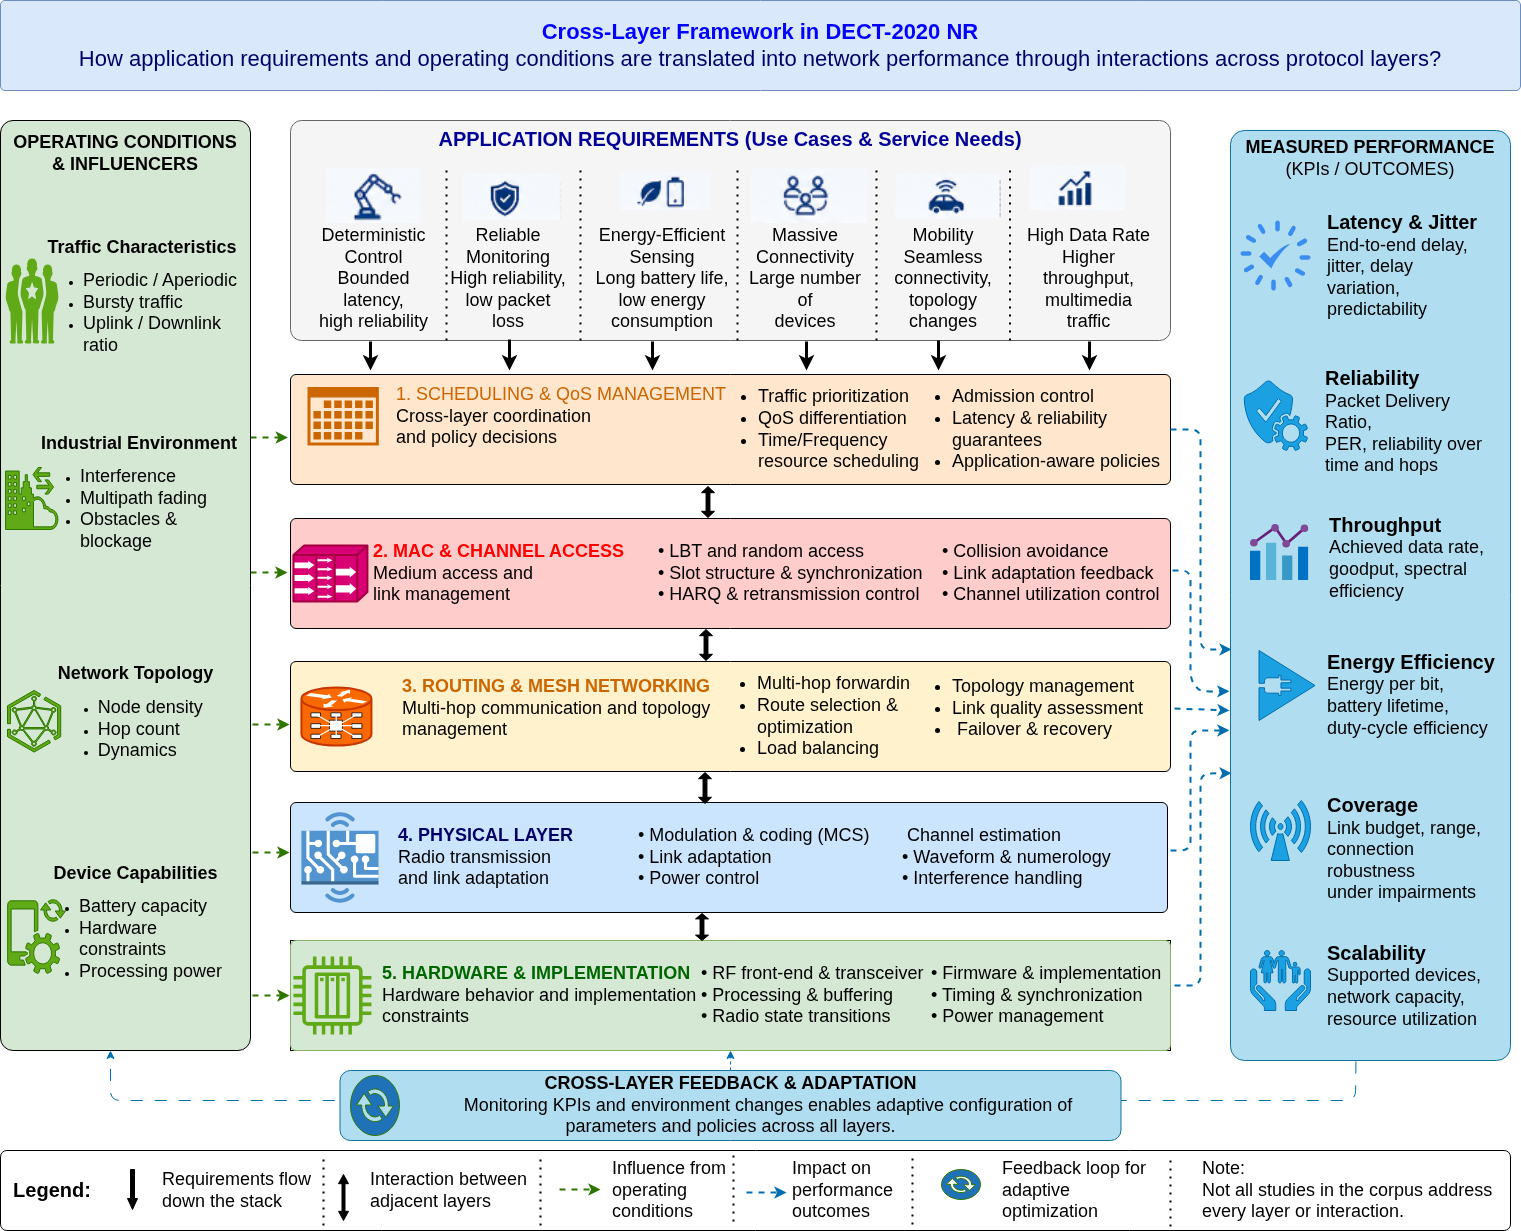
\includegraphics[width=\textwidth]{figures/CrossLayerFramework.png}
    \caption{Application-oriented cross-layer framework for DECT-2020 NR,
    illustrating how application requirements and operating conditions interact
    with scheduling, MAC, routing, PHY, and hardware mechanisms to determine
    measurable application-level performance.}
    \label{fig:cross_layer_framework}
\end{figure*}

This interaction is especially important for industrial applications because their requirements differ substantially. Periodic sensing may prioritize energy efficiency and long device lifetime, deterministic control requires bounded latency and high reliability, mobile systems introduce topology and routing dynamics, and professional media applications combine stringent timing with sustained traffic. Existing implementations demonstrate the feasibility of several such application classes \cite{mudriievskyiCHEAP5GDECT2024a, poetsProfessionalNetworkedAudio2025, piresDECT2020NREnergy2026b}, but the reviewed literature does not yet provide a systematic mapping from application requirements to complete PHY, MAC, scheduling, routing, and energy-management configurations.

This gap is particularly visible in scheduling and resource allocation. Although DECT NR+ provides flexible resource assignment and decentralized channel access, comparatively few included studies treat application-aware scheduling as their primary problem. Existing work demonstrates benefits from adaptive random access, coordinated resource configuration, and application-dependent PHY selection \cite{gaidamakaOptimizingDelaysRandom2025, glazkovImprovingNearURLLCServices2025, grafParetoOptimalityApproach2026a}, but joint management of deterministic, reliability-oriented, high-throughput, and energy-constrained traffic remains insufficiently explored in the reviewed literature. Future work should therefore move from isolated parameter optimization toward configurable cross-layer strategies that select operating points according to explicit application requirements and observed network conditions.


%%%%%%%%%%%%%%%%%%%%%%%%%%%%%%%%%%%%%%%%%%%%%%%%%%%%%%%%%%%%%%%%%%%%%%%%%%%%%%%%
\subsection{Experimental and Methodological Gaps}
\label{subsec:experimental_gaps}
%%%%%%%%%%%%%%%%%%%%%%%%%%%%%%%%%%%%%%%%%%%%%%%%%%%%%%%%%%%%%%%%%%%%%%%%%%%%%%%%

A second major limitation concerns the gap between the scale and abstraction of simulation studies and the conditions evaluated experimentally. Analytical and system-level studies frequently consider dense and multi-hop deployments, whereas physical experiments typically involve smaller device populations, point-to-point communication, or relatively simple static topologies. Recent multi-hop and application-oriented prototypes represent important progress \cite{piresDECT2020NREnergy2026b, poetsProfessionalNetworkedAudio2025}, but the reviewed literature provides limited evidence from large physical deployments combining routing, scheduling, heterogeneous traffic, mobility, and interference.

This distinction matters because physical implementations introduce effects that are commonly simplified or omitted in simulation. Radio-state transitions, processing and buffering delays, firmware behavior, synchronization, gateway processing, and transceiver turnaround can contribute directly to application-visible performance \cite{bandaraExperimentalValidationAnalysis2025, piresDECT2020NREnergy2026b, alizaiMeasurementDrivenLatencyAnalysis2026}. Protocol-level improvements should therefore increasingly be evaluated together with the implementation constraints of the target hardware.

Comparison across experimental studies is further complicated by the absence of common benchmark configurations. Payload size, MCS, transmit power, traffic load, topology, channel conditions, measurement duration, hardware platform, and even the boundaries used to define latency differ between studies. Consequently, apparently different performance results may reflect different experimental conditions rather than differences in the mechanisms being evaluated. A reproducible DECT NR+ evaluation framework should therefore report at least the PHY configuration, channel and bandwidth, transmit power, packet size, traffic model and offered load, number of devices, topology and hop count, interference conditions, firmware or modem version, and measurement duration.

The reported \glspl{kpi} also reveal a pronounced imbalance in the current evidence base. Packet loss or \gls{per} is evaluated in 40 of the 51 included studies, whereas energy or power is addressed in 22 and latency in 15. Reliability or outage also appears in 15 studies and \gls{ber} in 11, while coverage or range is evaluated in seven and throughput in five. In contrast, fairness, \gls{rssi}, and \gls{snr}/\gls{sinr} are reported in only two studies each, while \gls{aoi}, localization error, connection density, and spectral efficiency each appear in only one study. This distribution indicates that the literature has concentrated more strongly on link reliability and radio-level performance than on several application- and system-level properties.

For latency-sensitive industrial systems, average delay alone is insufficient because rare but large delays can determine whether application deadlines are satisfied. Future evaluations should therefore increasingly characterize latency distributions and high percentiles together with reliability, jitter, energy consumption, and application-specific performance measures. Such reporting would provide a more complete representation of predictability than mean values alone.

Long-duration and failure-oriented validation represents another important gap. Industrial networks must continue operating under interference, node failures, route changes, mobility, bursty traffic, and changing propagation conditions. Within the reviewed literature, comparatively limited evidence is available from long-duration experiments or controlled failure scenarios. Experiments extending over hours or days, together with controlled fault injection and recovery analysis, would therefore provide stronger evidence of system behavior under deployment-relevant conditions.


%%%%%%%%%%%%%%%%%%%%%%%%%%%%%%%%%%%%%%%%%%%%%%%%%%%%%%%%%%%%%%%%%%%%%%%%%%%%%%%%
\subsection{Research Gaps and Future Research Priorities}
\label{subsec:future_directions}
%%%%%%%%%%%%%%%%%%%%%%%%%%%%%%%%%%%%%%%%%%%%%%%%%%%%%%%%%%%%%%%%%%%%%%%%%%%%%%%%

The preceding analysis indicates that the next phase of DECT NR+ research should increasingly address how individual mechanisms interact within complete industrial systems. Table~\ref{tab:research_gaps} consolidates the principal gaps identified from the reviewed literature and maps them to corresponding research priorities.

\begin{table*}[!t]
\centering
\caption{Key research gaps and future research priorities identified from the
reviewed DECT-2020 NR literature.}
\label{tab:research_gaps}
\renewcommand{\arraystretch}{1.12}
\small
\begin{tabular}{p{3.0cm} p{5.3cm} p{7.0cm}}
\hline
\textbf{Research Area} &
\textbf{Identified Gap} &
\textbf{Future Research Priority} \\
\hline

Cross-layer and application-oriented design & The reviewed literature provides limited mapping from application requirements to coordinated PHY, MAC, scheduling, routing, and energy configurations. & Develop cross-layer configuration methods that translate latency, reliability, traffic, mobility, density, and energy requirements into coordinated protocol and radio parameters. \\

Scheduling and resource allocation & Application-aware scheduling under heterogeneous traffic and competing \gls{qos} requirements remains comparatively underexplored in the reviewed literature. & Develop deterministic and reliability-oriented scheduling and resource allocation for coexisting periodic, event-driven, bursty, and energy-constrained traffic. \\

Large-scale mesh networking & Large and dense networks are primarily evaluated analytically or through simulation, while physical multi-hop testbeds in the reviewed literature remain comparatively small. & Validate routing, topology management, scalability, mobility, congestion, and recovery using larger hardware deployments under realistic traffic and interference. \\

Experimental methodology & Experimental configurations, measurement boundaries, hardware platforms, and reported \glspl{kpi} vary substantially across the included studies. & Establish reproducible benchmark scenarios and standardized reporting of radio, traffic, topology, hardware, firmware, interference, and measurement conditions. \\

Reliability and deterministic communication & Latency and reliability are widely investigated, but the reviewed literature provides more limited evidence on tail behavior, predictability, failures, and sustained operation. & Evaluate latency distributions, deadline satisfaction, reliability, and recovery under interference, topology changes, retransmissions, failures, and long-duration workloads. \\

Energy-aware networking & The reviewed literature provides limited joint evaluation of energy with routing, reliability, latency, and network availability. & Jointly investigate PHY adaptation, sleep scheduling, router-role management, routing, residual energy, and application \gls{qos} to optimize network lifetime. \\

Positioning and localization & Positioning has received substantially less experimental attention than core communication mechanisms in the reviewed literature. & Validate integrated communication and positioning under industrial propagation, mobility, NLoS conditions, and realistic anchor deployments. \\

Security, coexistence, and heterogeneous integration & Security, coexistence, and multi-RAT operation remain comparatively less investigated and experimentally validated. & Investigate secure multi-hop operation, authentication, interference-aware coexistence, failover, and integration with Wi-Fi, cellular, and industrial networks. \\

Hardware-aware system design & Radio turnaround, processing, buffering, firmware, and other implementation-specific effects are not consistently represented in the reviewed system-level models. & Integrate hardware constraints into latency, scheduling, energy, and cross-layer models and validate the resulting designs experimentally. \\

\hline
\end{tabular}
\end{table*}

Several priorities cut across the individual areas in Table~\ref{tab:research_gaps}. Multi-objective configuration is required because improvements in latency, reliability, throughput, and energy can conflict \cite{grafParetoOptimalityApproach2026a}. Reliability-oriented mechanisms should increasingly be validated under mixed traffic and changing network conditions \cite{samuylovEmpoweringNearURLLCIoT2025, glazkovImprovingNearURLLCServices2025, ahmadMACLayerProtocolUltraReliable2025}, while energy-aware networking should combine router management, sleep behavior, routing, and radio configuration rather than treating transmit power in isolation \cite{nihtilaEnergyConsumptionDECT20202022, nihtilaEnergySavingRouter2022, grafParetoOptimalityApproach2026a}.

Areas with comparatively limited evidence also require broader experimental attention. Positioning studies demonstrate the potential of communication-assisted localization \cite{saikkoPositioningDECT2020NR2024, saikkoPositioningTrackingDECT20202025}, while primary studies on heterogeneous networking demonstrate practical integration of DECT NR+ with complementary radio and network infrastructures \cite{dangEWDCIntegratingDECT20202025a, dangUniRATUnifiedDECT20202026}. Related contextual work further illustrates a potential pathway for integrating resource-constrained devices with infrastructure-managed authentication and session management \cite{ngoIoTDeviceAuthentication2025}. These directions require broader evaluation under realistic industrial mobility, interference, security, and failover conditions.

Overall, the principal challenge identified by this review is no longer only to demonstrate that individual DECT NR+ mechanisms can achieve favorable performance, but to determine how they should be configured and combined to provide predictable application-level behavior under realistic scale, traffic, topology, interference, energy, and hardware constraints. Addressing this challenge through reproducible and increasingly large-scale experimental evaluation would strengthen the evidence needed to translate the flexibility of DECT NR+ into dependable industrial wireless systems.
%%%%%%%%%%%%%%%%%%%%%%%%%%%%%%%%%%%%%%%%%%%%%%%%%%%%%%%%%%%%%%%%%%%%%%%%%%%%%%%%
\section{Conclusion}
\label{sec:conclusion}
%%%%%%%%%%%%%%%%%%%%%%%%%%%%%%%%%%%%%%%%%%%%%%%%%%%%%%%%%%%%%%%%%%%%%%%%%%%%%%%%

This systematic literature review provides a structured synthesis of DECT-2020 NR research published between 2020 and July 2026. Following the PRISMA 2020 methodology, 51 primary studies were analyzed with respect to research characteristics, technical contributions, evaluation methods, experimental platforms, performance metrics, and application domains. The review shows a rapidly expanding research landscape, with approximately 75\% of the included studies published between 2024 and July 2026.

The evidence demonstrates substantial research activity in the PHY, MAC, and routing/mesh layers, accompanied by increasing experimental validation using commercial devices, SDR platforms, hardware prototypes, field measurements, and application-oriented testbeds. At the same time, scheduling and resource allocation, positioning, security, coexistence, heterogeneous integration, and large-scale experimental mesh evaluation remain comparatively less investigated. The reviewed studies further show that DECT NR+ performance cannot be characterized through individual protocol layers or isolated \glspl{kpi}. Radio configuration, channel access, scheduling, routing, topology, energy management, traffic characteristics, and hardware behavior interact to determine application-visible latency, reliability, throughput, coverage, and energy consumption.

A central finding of this review is therefore the need to move from isolated mechanism evaluation toward application-oriented cross-layer configuration and validation. Although simulation and analytical studies have established a broad understanding of DECT NR+ behavior, physical experiments remain comparatively limited in scale and frequently differ in hardware, traffic, topology, radio configuration, measurement duration, and performance definitions. Larger and more reproducible experimental studies are needed to evaluate heterogeneous traffic, multi-hop operation, mobility, interference, failures, long-duration behavior, and implementation-specific constraints under deployment-relevant conditions.

Overall, the reviewed literature indicates that DECT NR+ provides a flexible foundation for decentralized and industrial wireless communication, while its practical performance remains strongly dependent on application requirements and cross-layer configuration. Future progress will therefore depend not only on improving individual PHY, MAC, scheduling, or routing mechanisms, but also on understanding how these mechanisms should be coordinated and experimentally validated to provide predictable application-level behavior. Establishing reproducible benchmarks, application-oriented configuration methods, and larger-scale experimental evidence will be important for translating the technical flexibility of DECT NR+ into dependable industrial wireless deployments.

\section*{Acknowledgment}

During the preparation of this manuscript, the authors used ChatGPT (OpenAI) to assist with language refinement and improvement of the clarity and organization of selected passages. All technical content, references, results, interpretations, and conclusions were reviewed and verified by the authors, who take full responsibility for the final manuscript.

% ============================================================
% References
% ============================================================

\bibliographystyle{IEEEtran}
\bibliography{references}
\EOD

\end{document}